% % ME310 Report Template -- Started 28 July 2006  Mark Cutkosky
% % Updated: 7Aug08 -LMS; 25Nov10 Mark Cutkosky
% %%%%%%%%%%%%%%%%%%%%%%%%%%%%%%%%%%%

% % Rename this file to whatever you like (e.g. OurFallDoc.tex) and modify the title, authors
% % etc. below. If you rename the section files (e.g. Ch2context.tex) you'll need to change
% % the \include{ } calls in this document as well.

% %%%%%%%%%BEGIN DOCUMENT STYLE SETTINGS%%%%%%%%%%%
% % Don't modify this stuff unless you know what you're doing...
% % We are using the "memoir" class, a widely used set of macros book-like documents.
% % If you get errors that you are missing the "memoir" package you can download and 
% % install it:   http://www.ctan.org/tex-archive/macros/latex/contrib/memoir/

% % memoir document class for standard USA letter paper, printed one side
% \documentclass[11pt,letterpaper,oneside]{memoir}
% \chapterstyle{section}
% \pagestyle{companion}
% \usepackage{graphicx}        % standard LaTeX graphics 
% \usepackage{color}              % support for colored fonts
% \usepackage{url}  \urlstyle{same}     % deal with url strings in bibliography

% \usepackage[pdftex,           %hyperlink cross references, etc.
%     pdfsubject={ME310 Documentation},
%     colorlinks={true},
%     linkcolor={black},
%     citecolor={blue},
%     bookmarksopenlevel=1,
% ]{hyperref}                             

% %The file "me310.sty" should be in the same directory as this file.
% % It contains formatting for page setup, titlepage, glossary, references, etc.
% \usepackage{me310}           
% %%%%%%%END DOCUMENT STYLE SETTINGS%%%%%%%%%%

\documentclass[12pt,letterpaper,oneside]{memoir}

\chapterstyle{section}

\pagestyle{companion}

\usepackage{xeCJK}

\setCJKmainfont{AR PL SungtiL GB}

\xeCJKsetup{CJKglue=\hspace{0pt plus .08 \baselineskip }}

\usepackage{graphicx}

\usepackage{color}

\usepackage{url} \urlstyle{same}

\usepackage{me310}

\usepackage[%pdftex,           %hyperlink cross references, etc.
    xetex,
    pdfsubject={ME310 Documentation},
    colorlinks={true},
    linkcolor={black},
    citecolor={blue},
    bookmarksopenlevel=1,
]{hyperref}                             

\usepackage{setspace}

\linespread{1.4}

\raggedbottom
\usepackage{parskip}
\setlength{\parskip}{5pt}
\setlength{\parindent}{26pt}

%%%%%%%%%%BEGIN TITLE PAGE%%%%%%%%%%%%%%%%

%Replace the strings below with what's right  for you.

%%Insert your Document Title here. Use \\ to force a newline.

%\title{An Interactive Appliance\\
%for Individual Well Being}

\title{基于远程呈现机器人的\\
在线校园参观系统}

%%Enter your team members' names here:      
    \author{王照栋\\
    贾肇聪}

\team{远程呈现机器人组}            % Insert your Team Project Name here.

%% Insert Fall, Winter, Spring here:
\quarter{Fall Design Document}

%% If you don't want it to use the printing date, replace "\today"
%% with the date that you want.
\date{\today}
%%%%%%%%%%%END TITLE PAGE%%%%%%%%%%%%%


%%%%%%%%%BEGIN CUSTOM ABBREVIATIONS%%%%%%%%%
% Define any abbreviations that will apply throughout the document
% to save typing. Examples:
%\def\pmt{{\em Papier M\^{a}ch\`{e}}}  %Define "\pmt" to print "Papier Mache" with accents +1space
%\def\cbike{{\em Casterbike} \,}  %Define "\cbike" to print "Casterbike " italicized +1space
%%%%%%%%%END CUSTOM ABBREVIATIONS%%%%%%%%%

%%%%%%%%DRAFT COMMENTS%%%%%%%%%%%%%%%%
%Allow comments (remarks) to be shown or hidden.
% Put optional text in \begin{remark} ... \end{remark}  environments.
%The usage is a bit counterintuitive: \commentsoff makes them visible; \commentson hides them.
\commentson{remark} %Don't print remarks.
%\commentsoff{remark}  %Do print remarks. 


%%%%%%%%%%%%%%%%%%%%%%%%%%%%%%%%%%%%%%%%
%   BEGIN THE MAIN DOCUMENT
%%%%%%%%%%%%%%%%%%%%%%%%%%%%%%%%%%%%%%%%
\begin{document}

%If you want a figure on the cover page, this is where it goes.
%7 cm is about max figure height before messing up title spacing.
%If making your own fancy coverpage (e.g. in Photoshop) then comment out 
%the \includegraphics{ } and use the \vspace{ } command.
\begin{figure}[t]
% \centering
%   %An example cover image, from 2008 ME310 Kodak project
%   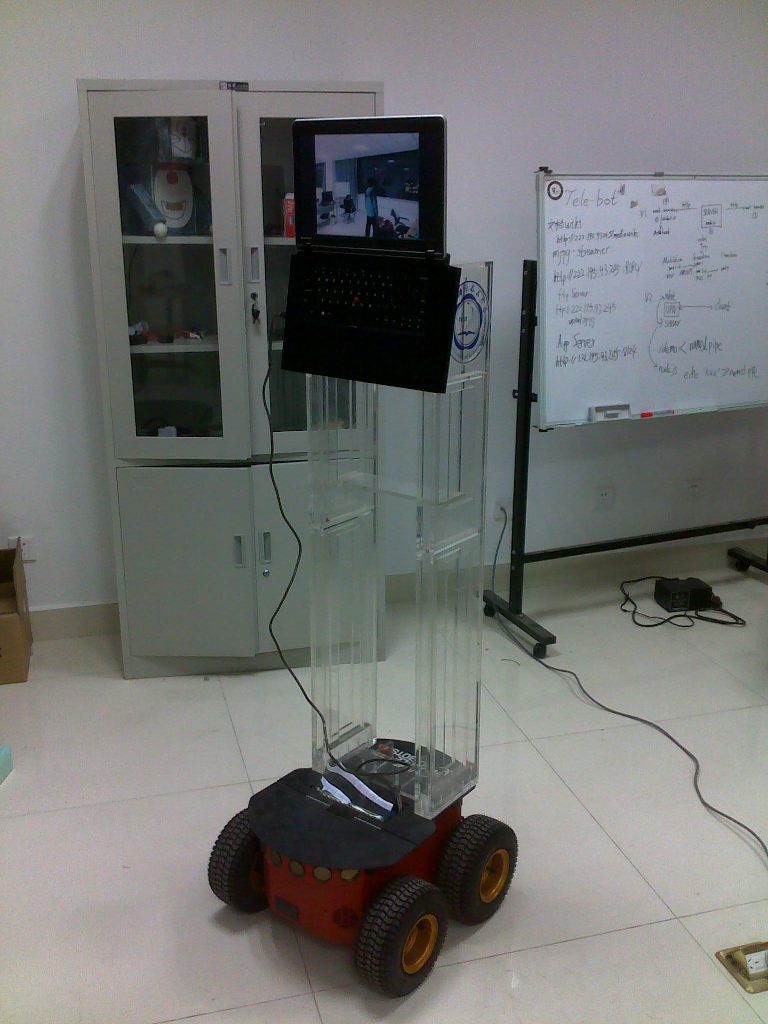
\includegraphics[height= 7cm]{Figures/cover.pdf}
\vspace{3 cm}    %Use this instead if you have no cover picture 
\end{figure}

%%%%%%%%%%%%%%%%%%%%%%%%%%%%%%%%%%%%%%
%Make the title page using arguments defined above.
\titlep

%%%%%%%%%%%%%%%%%%%%%%%%
% Load file "Executive.tex" for the Executive summary.
% Remember, this is a stand-alone section for executives to read.
%The executive summary is a special chapter before the TOC
% See the other sections (e.g. Context) for more normal chapter headings
%%%%%%%%%%%%%%%%%%%%%%%%%%%%%%%%%%%%
% Call it Front Matter in TOC, as it will include Glossary and auto-generated TOC, LOF.
\chapter[Front Matter]{摘要} 
\label{cha:front}
\addcontentsline{toc}{section}{Executive Summary}
%%%%%%%%%%%%%%%%%%%%%%%%%%%%%%%%%%%%
%Begin the actual executive summary text. If you create any subsections you
%probably want to use  \section*{Section name}  with an asterisk, so they are not numbered.
% Note: to get proper looking quotes use two left/right single quotes: ``. . . ''

%Example of a remark that can be optionally printed:
\begin{remark}\color{blue}
Suggested length of this section: 2 pages including figure(s).
\noindent This the most important section to edit carefully. It should stand alone. Assume it is the \emph{only} section that your corporate liaison's boss will read.
\begin{itemize} \tightlist   % a list with reduced white space
\item Introduce the reader to what your project is about. 
\item Say something brief about the design teams.
\item Motivate the current project direction. The motivation is based on findings from user and expert
interviews, benchmarking, CEP and CFP tests, etc. What interesting findings or insights do you have?
\item \textbf{What you did} is less important than \textbf{what you learned}.
\item Make sure your current ``Point of View'' comes across. The person who reads only the Executive
Summary should still have an idea who your User is.
\item Include one or two images that capture the gist of your design. For Fall, we're probably talking about
pictures of a proposal or vision rather than something you've designed. However, it's possible that something 
from your CFP, CEP or Benchmarking gets the idea across.
\end{itemize}
The remainder of this section is taken from \cite{Autodesk2008Fall}, a pretty good Fall document, done in Latex.
\normalcolor
\end{remark}
%End of remark

%%%%%%%%%%%%%%%%%%BEGIN EXAMPLE TEXT FOR THIS SECTION %%%%%%%%%%%%
\section*{Example text}

% Engineers must work with distributed teammates around the world. More than ever, designers are tackling all stages of design with remote coworkers whom they may never actually meet face to face. Functioning in this distributed environment can be very challenging both technically and socially. While there are many great tools for managing data and capturing concepts, sharing the output of these tools between distant teammates requires thoughtful planning and continued effort to include distant coworkers during the meeting. Also, distributed team members often feel a sense of isolation - studies have shown that people will collaborate more with people in the same room than with their distributed coworkers who are calling in \cite{Milnethesis}. Developing a way to level the playing field for distributed designers is essential for ever achieving effective distributed design.

在开放性较大的大学校园里,对环境陌生的人群往往需要一定的辅助来了解校园的设施、结构等信息。

\begin{figure}[h]
        \centering
                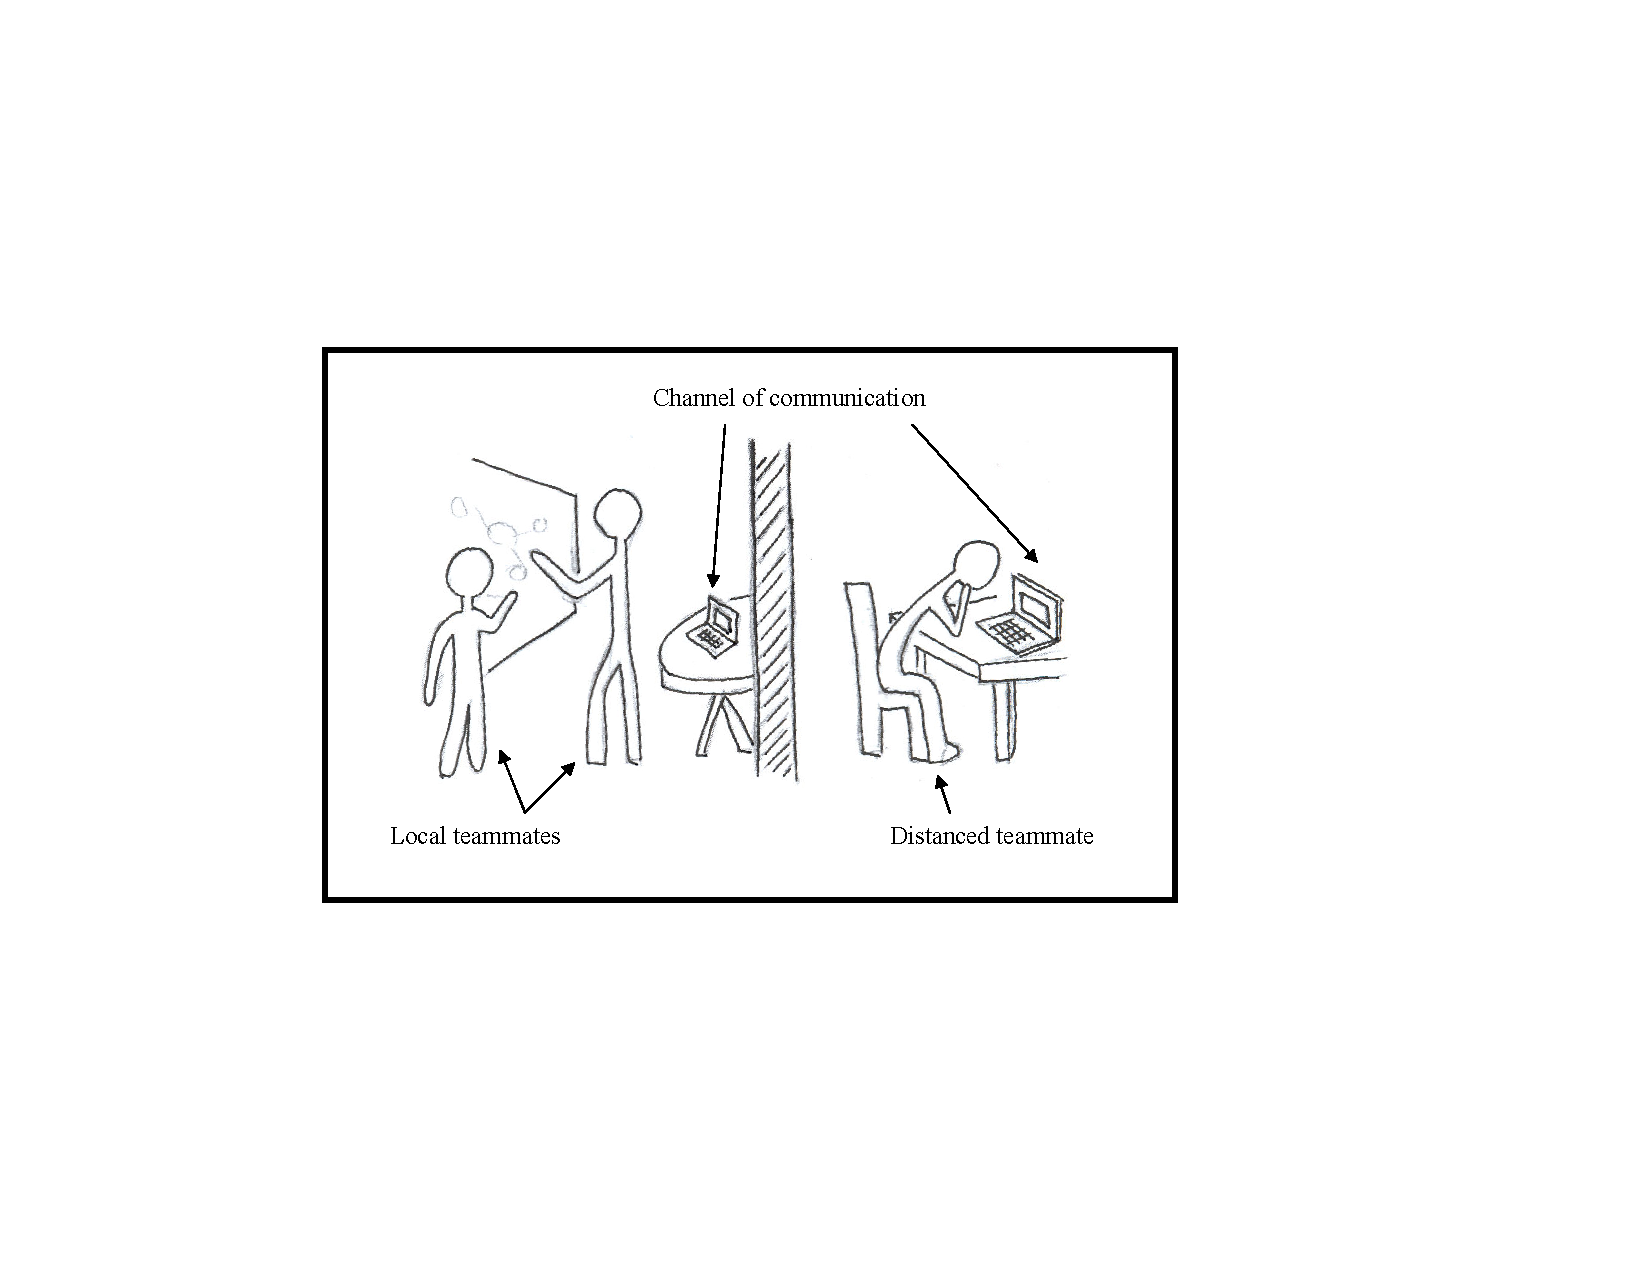
\includegraphics[width=.75\textwidth]{Figures/Ch1frontmatter/execimage.pdf}
        \caption{Common result of destributed design meetings}
        \label{fig:executive}
\end{figure}

 % Autodesk has approached our team of 3 engineering students at Stanford University and 3 engineering students at Pontificia Universidad Javeriana to tackle this issue of how to get engineers to collaborate better. To gain an understanding of what makes great collaboration, we have surveyed existing collaboration technology, talked with designers, and run scenarios for different collaboration environments. We focused on solutions for the early stages of the design process between small, distributed teams. 

% After researching a plethora of communication devices for sharing audio, displaying video and sharing drawings, we realized that the critical issue was not how to input drawings or video. The more pressing issues are how designers share the output of the tools and how to capture records of the information that is created. During the brainstorming phase, where ideas are generated quickly and randomly, finding a way to record a meaningful and accessible archive of concepts is especially difficult with existing collaboration tools.

% Another important component of obtaining improved group collaboration is getting people to work together as a cohesive group, be it a distributed team or not. How do you deal with the coworker who keeps dominating the conversation? How do you get that quiet person to be more involved? No one is responding to my idea, don't they like it? The team has hypothesized that applying one of the key tenants of improvisational acting could assist with these social frustrations - have a moderator. Dialogue is critical to successful brainstorming, and can potentially be facilitated by objective feedback from a third person observer.

% We also tested the ability of uncrowded channels to pass information without disturbing the flow of conversation. By prototyping a tactile feedback system, we found that it enabled a non-intrusive way to get someone's attention, and more importantly created a sensation of proximity with distributed teammates. 

就需求来讲,某个特定的场所可能有诸多的信息需要开放介绍,甚至需要对来访人员进行一定的导航、指引,而通过单一的静态信息可能无法达到较好的传递效果,以此为出发点,我们力图构建一个系统来改善诸如此类的信息展示功能。

对于这种有效信息的获取,其渠道是多元化的,在远程呈现的应用可能下,我们可以将其作为一种获取方式进行设计。让身处远方的“参观者”能够“身临其境”的感受环境,也即通过实时远程传递音频、视频等信息,并且让使用者“自主”的去寻找他们感兴趣的信息。同时,这种功能不只是单向的,通过远程呈现的平台,可以实现两地的人员的实时交流、咨询,也即实现一定的“虚拟出席”的功能,用以辅助环境信息获取的效率。

一个可以令人感兴趣的设计是一种集散控制的导航、参观系统。

旨在某一建筑物中配置一套机群,其移动终端为可移动的并且具有网络传输功能的“远程呈现机器人”,其基本功能是代替参观者虚拟出席到特定环境中,并获取基本的环境信息,对于移动性的控制,一方面可以由非现场的参观者通过某一指标(比如一张平面图的点击)来安全的(操作上存在一定的必要限制)控制移动,另一方面可以由现场人员在移动终端上直接输入指令进行辅助控制,该辅助控制也可以通过前述的平面图点击来封装化的实现。

这一套散布式机群的远程命令获取,是通过一台服务器的命令转发来实现的,用
户通过网络与服务器建立连接,发送给定的指令,服务器负责将指令集中,转发
到分散的特定的远程呈现机器人终端,这一设计便是集散式的系统分部。

\begin{figure}[h]
        \centering
                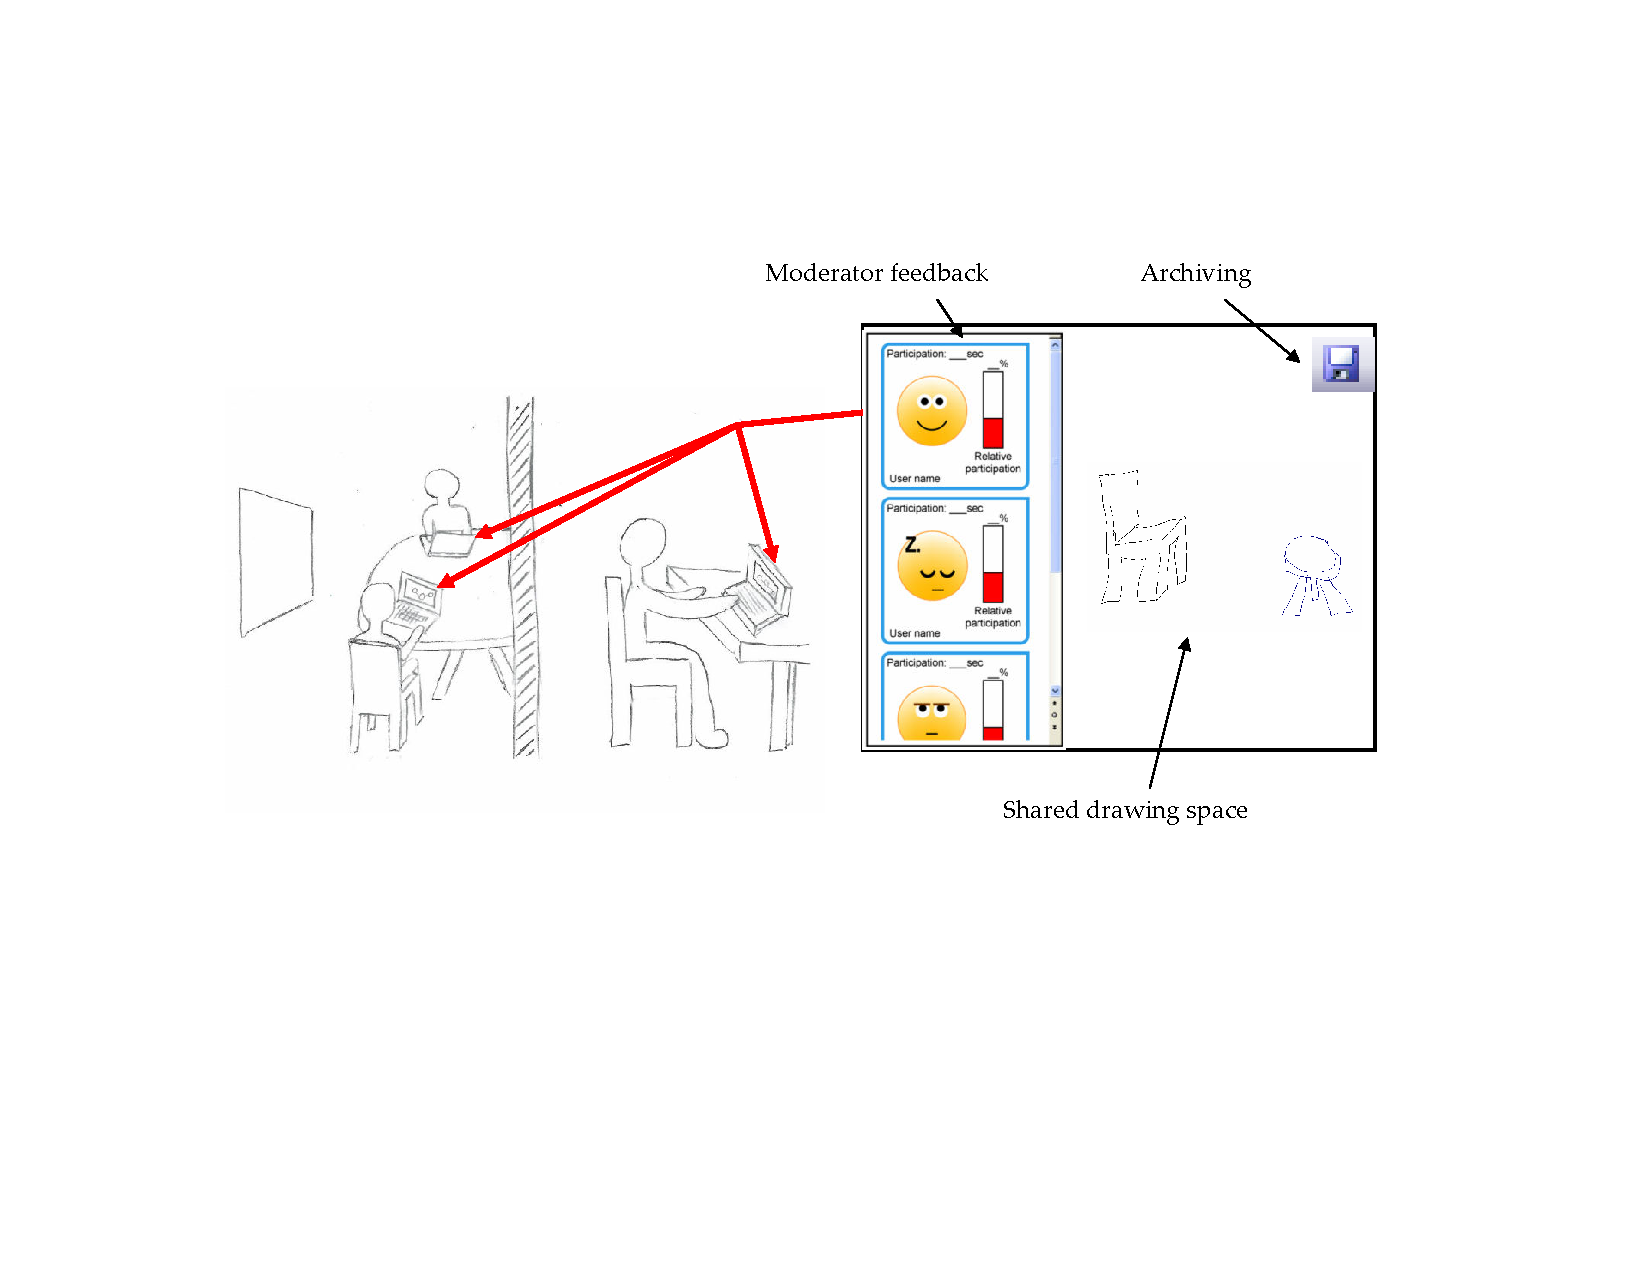
\includegraphics[width=.75\textwidth]{Figures/Ch1frontmatter/execimage2.pdf}
        \caption{Vision for a more effective distributed design meeting}
        \label{fig:execimage2}
\end{figure}

% A vision for the final product is to better enable dialogue by displaying explicit teammate feedback and participation level visible to the team. Imagine knowing when someone wasn't paying attention, or that your teammate thought you were talking too much, or that everyone really thinks you're idea is pretty cool. All of this could be displayed without saying anything. Aside from simply providing a platform to share information, the system will monitor the quantity of inputs and determine individual participation level, and also offer the opportunity for direct feedback. The objective is to  provide a real-time answer to a common wonder -  what are my teammates really thinking?  

%%%%%%%%%%%%%%%%%%END EXAMPLE TEXT FOR THIS SECTION %%%%%%%


\begin{remark}\color{blue}
\section*{Latex tips:}
\begin{itemize}\tightlist
\item These remarks in blue disappear if you select \textbackslash commentson\{remark\} in me310report.tex
\item Some teams will find the default report cover sheet too plain and will want to change fonts and layout, etc. This is a tedious in Latex. Use Powerpoint or Photoshop or other program to make a nice outer cover which you can pre-pend to the PDF file from Latex.
\item References are linked using the``cite'' command. The template is currently set up to use a bibliography style sheet ``plainurl310.bst'', which is close to the style used by IEEE and other journals with citation numbers in square brackets (e.g., [1]) and printed alphabetically in the Bibliography section. The modifications provide for printing a URL (if there is one) for each reference in a plain format. Numerous other bibliography styles are available, although many do not work with URLs.
\end{itemize}
\normalcolor \end{remark}


%%%%%%%%%%%%%%%%%%%%%%%%
% TOC and LOF are automatically generated
% Make Table of Contents title smaller than a normal Chapter heading:
\renewcommand{\chaptitlefont}{\normalfont\Large\bfseries}
\newpage
\tableofcontents*  %asterisk to prevent it from getting a number

% Optional Lists of Figures and Tables:
\newpage
\listoffigures*  %Note that for this you probably want to add the [short-headings] to captions.
%\listoftables  %I decided to omit the LOT in this example.

%Back to normal size for subsequent sections
\renewcommand{\chaptitlefont}{\normalfont\Huge\bfseries}
%%%%%%%%%%%%%%%%%%%%%%%%

% Set up the Glossary. The template is looking for a file called
% "glossaryterms.tex" with glossary terms and definitions.
% You can either edit this file manually or you
% can use the Memoir glossary feature in which you insert items like
%   \glossary{glossary term}{our definition of what the term means}
% wherever you like, as you write your documentation.
% When you run the report through Latex, it will create a ".glo" file like
% "OurFallDocument.glo" which you can edit to create the file "glossaryterms.tex"
% There is also perl script I made which will do the formatting for you. 
%  perl Glo2Tex OurFallDocument.glo > glossaryterms.tex
\newpage
\section*{缩略词}
\addcontentsline{toc}{section}{缩略词}
\label{sec-glossary}
\begin{description}
% \item [3d audio technology] Simulation that creates the illusion of sound sources placed anywhere in 3 dimensional space, including behind, above or below the listener.
% \item[action-event control] Process where a user action creates an physical event.
% \item [API] Application Programming Interface.
% \item[array of microphones] Microphones linked together to expand the effective coverage area. 
% \item [Ausim] 3D audio hardware company.
% \item [Automatic beam steering] Signal processing technique to narrow the microphone coverage area. Used to pick out a speaker and suppress background noise coming from directions other than that of the speaker.
% \item[Benchmarking] A process of researching and observing to understand the state of the art for a given field or topic.
% \item[Brainstorming] A process by which groups of people generate ideas
% \item [Brainwaves] A common term that refers to post-synaptic potentials measured from many neurons in the brain
% \item [CDR] Center for Design Research at Stanford University
% \item [CFP] Otherwise known as a Critical Function Prototype, this is a prototype built to test a concept that is critical to addressing the problem statement.
% \item [Client] Computer program that accesses a server.
% \item [Client-server paradigm] A computing architecture which separates the client from a server over a computer network. 
% \item [Crowded channel] A communication channel that is clogged with information.
% \item [CVE] Acronym for Collaborative Virtual Environment. This is a virtual environment that support more than one user at the same time.
% \item [Dark Horse] An idea that is unlike the others preceding it, an outlier.
\item [远程呈现(telepresence)] 是一种虚拟实在,能够使人实时地以远程的方式于某处出场,即虚拟出场。此时,出场相当于"在场",即你能够在现场之外实时地感知现场,并有效地进行某种操作。

\item [集散控制系统(Distributed control system)] 是以微处理器为基础的对生产过程进行集中监视、操作、管理和分散控制的集中分散控制系统,简称DCS系统。
   % input the list "glossaryterms.tex"
\end{description}

%%%%%% Example of an optionally printed "remark"
\begin{remark}
\color{blue}
It's a sign of a successful team that the glossary becomes extensive. Define any non-obvious or invented terms. For example, if you reference something by an acronym, that might be a glossary term. Teams also coin terms to describe design features. Define such terms here.  Don't define obvious stuff (axle, keyboard).  

See comments in me310report.tex if you want to generate a glossary semi-automatically from tagged keywords.
\normalcolor
\end{remark}


%%%%%%%%%%%%%%%%%%%%%%%%%%%%%%%%
%% On to the main sections....  Just comment out the \input{} line
%% for any chapters that aren't ready yet.
%Context
\chapter{背景介绍}
\label{sec-context} %Label for cross-referencing

%%%%%%%%%%%%
\begin{remark} \color{blue}
Suggested length: About half a page each for the Need Statement and Problem Statement (plus figures, if any). Another page or two for the design team.
\vspace{0.1in}

\noindent The Context provides background and motivation for your project. It is an enlarged version of the brief context in your Executive Summary.  
\begin{itemize} \tightlist
\item Who came to you with a proposed project area? 
\item What background or context set the stage for your Needfinding and Benchmarking, activities?
\end{itemize}
\normalcolor \end{remark}
%%%%%%%%%%%%

\section{需求陈述}
\label{sec:need}

%%%%%%%%%%%%
\begin{remark} \color{blue}
This section is the high-level result of your user need-finding. It defines the ``Point of View'' or hypothesis that guides your ongoing work. 
\begin{itemize} \tightlist
\item Who wants or needs your product? Why do they want it? Or, what need does the product area address? 
\item What evidence do you have to substantiate the need? Use citations or other evidence you've gathered.
\end{itemize}
\noindent The remaining text is taken from \cite{Autodesk2008Fall}.
\normalcolor
\end{remark}
%%%%%%%%%%%%

% The design world has changed dramatically in the last decade. The widespread advancement and usage of digital prototyping tools has made it simpler and faster to realize new ideas. At the same time, globalization is requiring designers from remote locations to combine their ideas and make design decisions. 

% With the advancement of computational power and communication speed, digital prototyping tools have made it possible to transmit complex drawings around the world. Most digital tools that promote remote collaboration target the idea-to-conception stage of development. The early ideation stages of engineering design, however, are still more effective when discussed locally. The problems of effective communication and effective decision-making in this setting are still largely unsolved. Internet tools setup the virtual meeting space, yet communication is still not as effective as meeting in the same room. Often meeting participants cannot truly work together as they do face-to-face.

% Wouldn't it be perfect to have a new tool that focused on the interaction aspects of remote collaboration? A tool that made communication effortless, as if the participants were in the same room. Such a tool could increase the ideation potential of remote meetings and make remote brainstorming a reality. 

随着计算机、互联网技术的飞速发展,人与人、人与事物之间的联系日益密切,人们所接触的范围也逐渐广泛起来,于此同时,所需要的信息流量也会大大增加,传统的传递方式也许并不能很好的起到传递效果。如果让数字化介入其中,便会收获更好的结果。

试想一下,当某一个机构或部门需要向外界介绍他们的相关信息,这些信息会给参观者留下非常重要的印象,如果诸如此类的信息能够具有实时性、全方位性,并且能够充分调动参观者的主观感受,那么这些信息的价值便会大大提升。

通过远程呈现的基本构架,借助移动机器人提供的主观能动性,搭建如此的一个集散控制的参观导航系统,便会具有如上所述的极佳的效果。

当你身处千里之外,通过简单的互联网界面,点击鼠标、敲击键盘,就可以达到参观目的地的效果,而且这种信息的获取是实时动态的,该是一件多么惬意的事情,你一定会对目标地点有一个非常好的主观印象。而且,你还可以随时与那里的工作人员等互动交流,岂不是更加便捷、实用!

\section{问题陈述}
\label{sec:problem}

%%%%%%%%%%%%%%%
\begin{remark} \color{blue}
Here you get more specific about the particular problem that your design vision is addressing.
The remaining text is again taken from \cite{Autodesk2008Fall},
\normalcolor
\end{remark}
%%%%%%%%%%%%%%%

%In order to facilitate remote collaboration in the early design stage, we first break down the problem into the following three areas.

进一步分析目标,我们可以将过程中需要着重注意、解决的难题归纳总结,分成不同的项目部分,以备后续逐步实现预订功能。如下为分类:

\begin{itemize} \tightlist
\item 网络连接搭建的方式

\item 远程操作者的使用界面

\item 机器人上的用户界面

\item 机器人的操控方式

\end{itemize}

% Early ideation is a very social process and requires effective interperson communication. Current teleconferencing tools lack in recreating the level of social dynamics present in face-to-face communication.

% Communication tools are a means with which we transmit ideas to each other. This could be either through speaking, body language, or drawing. The early ideation stage requires a rapid exchange of ideas between all participants in a meeting. How can we utilize communication tools effectively to make such a dialog easier?

% Finally, the brainstorming stage presents a plethora of ideas that need to be archived and categorized for effective decision making. How can we make it easier for meeting participants to save their ideas and retrieve them later? How can information be viewed to facilitate decision making?

对于网络搭建,由于机器人可能部署在任意的网络环境中,因此不能对实现这套
系统的网络有过高的要求与假设。我们的设计目标是部署在机器人上的客户端无
需公网地址段的ip,也无需和使用者处于同一个子网内,只要机器人有一个无线
网络连接,就可以正常工作。

对于使用界面的设定,考虑到跨平台的潜在需求和移动互联网的趋势,应该采用基于网页界面的设计,具体的功能模块后续的设计中会逐渐添加,进而集成到界面中,以达到符合用户使用需求的目标。

机器人的控制方式也是一个非常重要的方面,它直接关系到了机器人的安全性等强制性的因素,而且对于用户体验也是至关重要的。

% \section{Autodesk}
% Since 1982, Autodesk has delivered 2D and 3D visualization tools for clients in manufacturing and design. Some products include the drafting program AutoCAD, digital prototyping software Inventor, and 3D modeler Maya. The company focuses on enhancing the design process by allowing the customer to experience their design through software.

%%%%%%%%%%%%%%%%%%%%%%%%%%%%%%%%%%%%%%%%%%%%%%%%%%

\section{组员介绍}
\label{sec:team}

%%%%%%%%%%%%%%%%%%%
\begin{remark} \color{blue}
See other recent reports for other ways of introducing the team. To the extent that the characteristics of the team influence the project direction, this is of interest to the reader.
\end{remark} \normalcolor
%%%%%%%%%%%%%%%%%%%

% Team \pmt, was assembled by the ME310 teaching staff, based on the outcome of Myers-Briggs personality tests (see Table \ref{wildeprefs}) and a desire to create teams with a diversity of interests and backgrounds. There is some evidence that such diversity enhances team creativity \cite{Wilde97} \cite{Wilde07}, even if it creates additional challenges for team management.

% Example table. It gets a caption and reference label.
% The tabular formatting is a bit painful...  An alternative is to use Word
% and insert the PDF printout as for a figure. There are also Word-to-Latex converters.
% \begin{table}
%   \begin{tabular}{| p{14mm} | p{20mm} | p{20mm} | p{22mm} | p{20mm} | p{12mm} |} 
%   \hline
% Score & Extroverted-Introverted (E-I) & Intuition-Sensing (N-S) & Feeling-Thinking (F-T) & Perception-Judging (P-J) & Overall \\
% People & & & & &\\
% \hline
% Eric & +6 & +6 & -6 & +12 & ENTP \\
% Azin & -18 & +30 & -30 & +18 & INTP \\
% Patrick & +6 & +18 & -18 & +6 & ENTP \\
% Salil & -18 & +30 & -30 & +18 & INTP \\
% \hline
% \end{tabular}
% \caption{Team preferences scores using the method of Wilde \cite{Wilde07}. }
%         \label{wildeprefs}  %Tag for referring to table
% \end{table}

% \begin{framed}
% \noindent 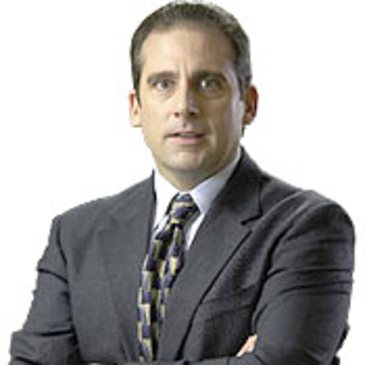
\includegraphics[width=50mm]{Figures/Ch2/Scott}
% \parbox[b]{0.6\textwidth}{Michael Scott\\
% Status: M.E. Graduate Student\\
% Contact: mscott@me310.stanford.edu\\
% Skills: mechatronics, welding, CNC machining\\
% Computing: Solid Works, Matlab, basic C programming, Flash, Dreamweaver\\
% }

% Born in Paris and raised in New Jersey, I attended Columbia University. For graduate school, I decided to trade in the hustle and bustle of New York City for the sunshine of Palo Alto, and so far I have not been disappointed (though New York will always be dear to my heart). My interests include mechatronics, design (including medical devices), football, tennis, pick-up games, tail-gating, Entourage, South Park.
% \end{framed}

\begin{framed}
\noindent 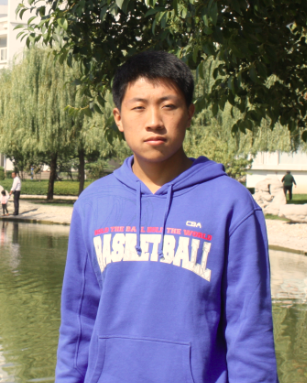
\includegraphics[width=50mm]{Figures/context.pic.png}
\parbox[b]{0.6\textwidth}{王照栋\\
现况:中国科学技术大学,自动化系,10级本科生\\
邮件:wangzd@mail.ustc.edu.cn\\
技能:基础机械结构设计,自动控制\\
编程:C语言编程,初步C++面向对象编程,matlab\\
}

来自山东,2010年考入中科大信息学院,后就读于自动化系。喜欢设计,并且具有一定的动手能力,2012年暑期与同学组队参加过Robogame机器人大赛,并最终获最佳技术奖单项奖。课余时间比较喜欢参与一些运动以及益智类的活动,热爱乒乓球、篮球、羽毛球、游泳等运动,对魔方速拧还原有一定的研究。
\end{framed}

\begin{framed}
\noindent
%\parbox[b]{0.6\textwidth}
{贾肇聪\\
现况:中国科学技术大学10级少年班学院\\
}
自由软件爱好者,在本项目中负责linux服务器的管理和网络维护。
\end{framed}

%%%%%%%%%%%%%%%%%%MORE LATEX EXAMPLES%%%%%%%%%%%%%%
% Let's test some in-situ glossary items. The idea is to insert these kinds of definitions anywhere,
% as they occur to you while incrementally working on the documentation.
%See main file for notes about how to convert the ".glo" file to a glossary section.

% \glossary {paper weight}{ the combined weight of all paper products (paper, cardboard, crepe paper, paper tape) in the vehicle.}
% \glossary {non-paper weight}{ the combined weight of all non paper items (e.g. metal pins, teflon tape, screws). Non-paper weight is severely restricted in ME310 Paper Bike exercises.}
% \glossary {papier m\^{a}ch\`{e} }{a composition of shredded paper glued together with library paste}
% \glossary {particle board} {a product made of compressed wood chips and resin, often sold in 4 ft x 8 ft sheets. Particle board is not considered a paper product.}
% \glossary {sound deadener board} {a product made of compressed cardboard fibers and resin, often sold in 4 ft x 8 ft sheets. Sound deadener board is not considered a paper product.}

\begin{remark} \color{blue}
\section*{Experiments with tables in Latex}

Here is a centered tabular form that is 3/5 of the current text width and has a horizontal line but no
vertical lines:

 \begin{center}  % put inside center environment
  \begin{tabular*}{0.6 \textwidth}%
     {@{\extracolsep{\fill}}cccr}
  \multicolumn{3}{c}{a label spanning 3 merged cells} & label 4  \\
  \hline  % put a line under headers
  item 1a  & item 2a  & item 3a  & item 4a  \\
  item 1b  & item 2c  & item 3c  & item 4c  \\
  \end{tabular*}
  \end{center}

\noindent For anything more complicated than the examples in this section, it may be easiest to do the table in MS Word or OpenOffice, create a pdf and include the pdf in a table environment, as done in Table \ref{tab:physical-requirements}. Because pdf files have scalable fonts, the print resolution will be good.

\end{remark}\normalcolor
 

%%%%%%%%%%%%%%%%%%%%%%%%%%%%%%%%
%%Design Requirements Chapter
\chapter{设计需求}
\label{sec-requirements}

\begin{remark} \color{blue}
Articulating design requirements is a critical task for a team that starts with a broad problem and needs to determine \emph{what they should design}. After need-finding, and technical and user benchmarking, the team proposes a {\em class of design solutions} that fulfill {\em requirements}\, associated with the problem. In the Fall document, the initial Requirements Definition is the main item of value that teams can deliver to sponsors.

As the design process continues, requirements become more concrete and detailed. New {\em de facto} \, requirements are discovered and documented. Ultimately, competing designs are evaluated with respect to the requirements. If you can't tell whether a design satisfies the requirements, the requirements are too vague.

It is suggested to follow the procedure introduced in Fall quarter lectures and the Paper Bicycle Documents for defining and organizing requirements:
\begin{itemize}\tightlist
\item Requirements (04 Oct. 2011): \url{https://www.stanford.edu/class/archive/me/me310a/me310a.1122/cgi-bin/mediawiki/index.php/FallCalendar} and handout on CloudSafe file server.
\item Paper Bicycle Docs: \url{https://www.stanford.edu/class/archive/me/me310a/me310a.1122/cgi-bin/mediawiki/index.php/PaperBikeDocumentation}
\end{itemize}
\normalcolor
\end{remark}

%This table can  be copied & pasted in your document. The fussy formatting is already set up correctly.
%To get wrapped text, you have use p{} and specify paragraph widths (total < 148mm)
% \begin{table}
% \color{blue}
%   \begin{tabular}{| p{44mm} | p{49mm} | p{42mm} |}   %3 columns, wrapped text
%   \hline
%   Requirement & Metrics & Rationale \\
%   \hline
%   a brief description of what the requirement or objective is & 
%   measurable quantities associated with requirement (how to assess if a design satisfies the requirement) &
%   why this requirement is important or valid \\

% % This example table can be copied and pasted with the text adjusted to meet your needs. &
% % Each column is separated by an ``\&'' sign. The text entries can wrap to more than one line if needed. &
% % Each row is separated by two backslashes and an optional horizontal line. \\
%     \hline
%   \end{tabular}
% \caption[Three column requirements format]{Three column format suggested for requirements (One can make a separate table for each cluster of related requirements).}
%         \label{threecolumnreqs}  %Tag for referring to table
% \normalcolor
% \end{table}

%The remainder of this section contains sample requirements (not an exhaustive set but enough to give an idea) from Autodesk Fall 2007-08 \cite{Autodesk2008Fall} and Audi Fall 2008-09 \cite{Audi2009Fall}.

%%%%%%%%%%%%%%%%%%%%%%%%%%%%%%%%

\section*{简介}

The Autodesk collaboration tool must enhance communication between groups of distributed engineers as they engage in brainstorming.  We have focused on enabling this collaboration via tools that:

\begin{itemize}\tightlist
\item Enable users to communicate naturally and through multiple channels.
\item Enable the team to better utilize their teammates, be they local or distant.
\item Capture the information that was presented.
\end{itemize}

Our benchmarking and prototyping efforts have led to a more detailed definition of what the product needs to be in order to successfully achieve this.  The requirements address what the product functionally needs to do and what it physically needs to be. Because of the wide range of functional opportunities that exist for the product, few physical restrictions are imposed at this stage in the design. 

\section{功能需求}
\label{sec:functionalreqs}

\begin{table}[!h]
        \centering
                \begin{tabular}{| p{42mm} | p{42mm} | p{51mm} |}
                \hline
                \textbf{Requirement}    & \textbf{Metrics} & \textbf{Rationale}\\
                \hline
The product will balance the number of interactions in distributed design meetings among the team members. &    Interactions are questions or statements that develop a concept. The total number of interactions per person during a design meeting will be called $n_{i}$. The solution must reduce the standard deviation of $n_{i}$ between team members as compared to the closest publicly-available competing product.   & The number of times someone interacts in a meeting is one measure of engagement. Brainstorming is a highly social process which thrives on the input from a variety of perspectives. By effectively improving the communication between distributed teams, team members will be more engaged and participate more.\\
\hline
                \end{tabular}
        \caption{Requirement for improved communication}
        \label{tab:mediums1}
\end{table}

\begin{table}[!h]
        \centering
                \begin{tabular}{| p{42mm} | p{42mm} | p{51mm} |}
                \hline
                \textbf{Requirement}    & \textbf{Metrics} & \textbf{Rationale} \\
                \hline
The solution must transmit sound at close to the rate of normal conversation. & The listener must hear the speaker with less than 0.3 seconds lag.      & Audio latency creates a sense of distance. Mobile phone to mobile phone conversations have an average latency of 0.3 seconds, which is noticeable but not disruptive. \\ \hline
Users can capture drawings to share with distributed teammates that are legible. &      Input device must be able to resolve a drawing at 50 points per inch (specifically, they must capture 50 percent contrast modulation at this frequency). &      Drawings by mechanical pencil and ball point pens typically have lines of 0.5mm thickness, which translates to a resolution of 50 points per pinch (ppi).\\ \hline
Users will be able to capture drawings to share with distributed teammates without disrupting the flow of the discussion. & Drawings must be captured and sent within 17 seconds. This is assuming the input device is properly set and there are no external complications. &  We found through benchmarking that sketches are used primarily when describing a concept, and are of little use afterwards. The sketches must be captured and sent before the context of the discussion has changed. Seventeen seconds was found to be about the average comment length during brainstorming in our prototyping. \\ \hline
Users will be able to see the drawings clearly. &       Drawings must be displayed with a resolution of at least 72 ppi.&       The display must be able to resolve at least as a standard computer monitor.\\ 
\hline
                \end{tabular}
        \caption{Required mediums of communication for effective concept development}
        \label{tab:mediums2}
\end{table}

\begin{table}[!h]
        \centering
                \begin{tabular}{| p{42mm} | p{42mm} | p{51mm} |}
                \hline
                \textbf{Requirement}    & \textbf{Metrics} & \textbf{Rationale} \\
                \hline
The tool must be able to be started up quickly for impromptu meetings.  & It must be able to be started in less than 40 seconds. This time is calculated from the moment someone decides to start the system, to the point when the tool is ready to use, with full functionality. If the solution requires use of personal laptops, assume these are already booted up. & Our benchmarking has shown that collaboration tools can fall into disuse if it requires a lengthy setup time. This amount of time is within the range of initiation times for multiple popular conferencing solutions. \\ \hline

        \end{tabular}
        \caption{Social requirements for effective design meetings}
        \label{tab:mediums3}
\end{table}



\newpage

\subsection{功能限制}

\begin{table}[!h]
        \centering
                \begin{tabular}{| p{44mm} | p{49mm} | p{42mm} |}
                \hline
                \textbf{Requirement}    & \textbf{Metrics} & \textbf{Rationale} \\
                \hline
                The bandwidth required must not be prohibitive to standard engineering offices. & The product will require less than 100 Mbps.& The population of potential users would dramatically decrease if the product required more connectivity than a T1 line, which is typically around 100 Mbps.\\ \hline
                        \end{tabular}
        \caption{Functional constraints}
        \label{tab:fconstraints}
\end{table}


\subsection{机遇}

\begin{itemize}\tightlist
\item Utilize existing tools. There are many collaboration and input  tools that exist out there. Our product does not need to be a replacement for them. It could potentially supplement them.
\item Offer new lines of communication:
        \begin{itemize}\tightlist
                \item Facilitate side conversations between distributed users.
                \item Utilize the uncrowded channels offered by other senses than audio/visual, such as tactile.
\end{itemize}
\newpage
\item Be the moderator: 
\begin{itemize}\tightlist
                \item Collect feedback from users directly, via voting, or indirectly. Enable the replacement of video, which conveys very little useful feedback during design meetings.
                \item Encourage the participants to be engaged by monitoring participation.
                \item Display feedback and participation to attendees non-verbally,potentially through the use of avatars.      
\end{itemize}
\item Allow for easier information capture and storage
\begin{itemize}\tightlist
                \item One button information capture
                \item User-driven archiving
\end{itemize}
\item Assist user communication in non-native languages.
        \begin{itemize}\tightlist
                \item Audio buffering
 \end{itemize}
\item The product should be accessible
\begin{itemize}\tightlist
\item Usable for low bandwidth connections for 
\item Be fast to setup.
\item Able to be setup within a typical conference room.
\end{itemize}
\end {itemize}

\subsection{假设}
\begin{itemize}\tightlist
\item Each user has, and is able to use:
\begin{itemize}\tightlist 
\item a personal laptop
\item a mouse
\item a microphone
\end{itemize}
\item Users will speak with a volume of at least 30 dB, as measured when 1 meter from the microphone.
\end{itemize}

%%%%%%PHYSICAL REQUIREMENTS%%%%%%%%%%%
\section{物理需求}
\label{sec:physicalreqs}

\color{blue}
For variety, here is a requirements table from an Audi fall document \cite{Audi2009Fall} done in MS Word and pasted as PDF into Latex. Notice that the fonts are scalable if you zoom in.
\normalcolor

\begin{table}[h]
        \centering
                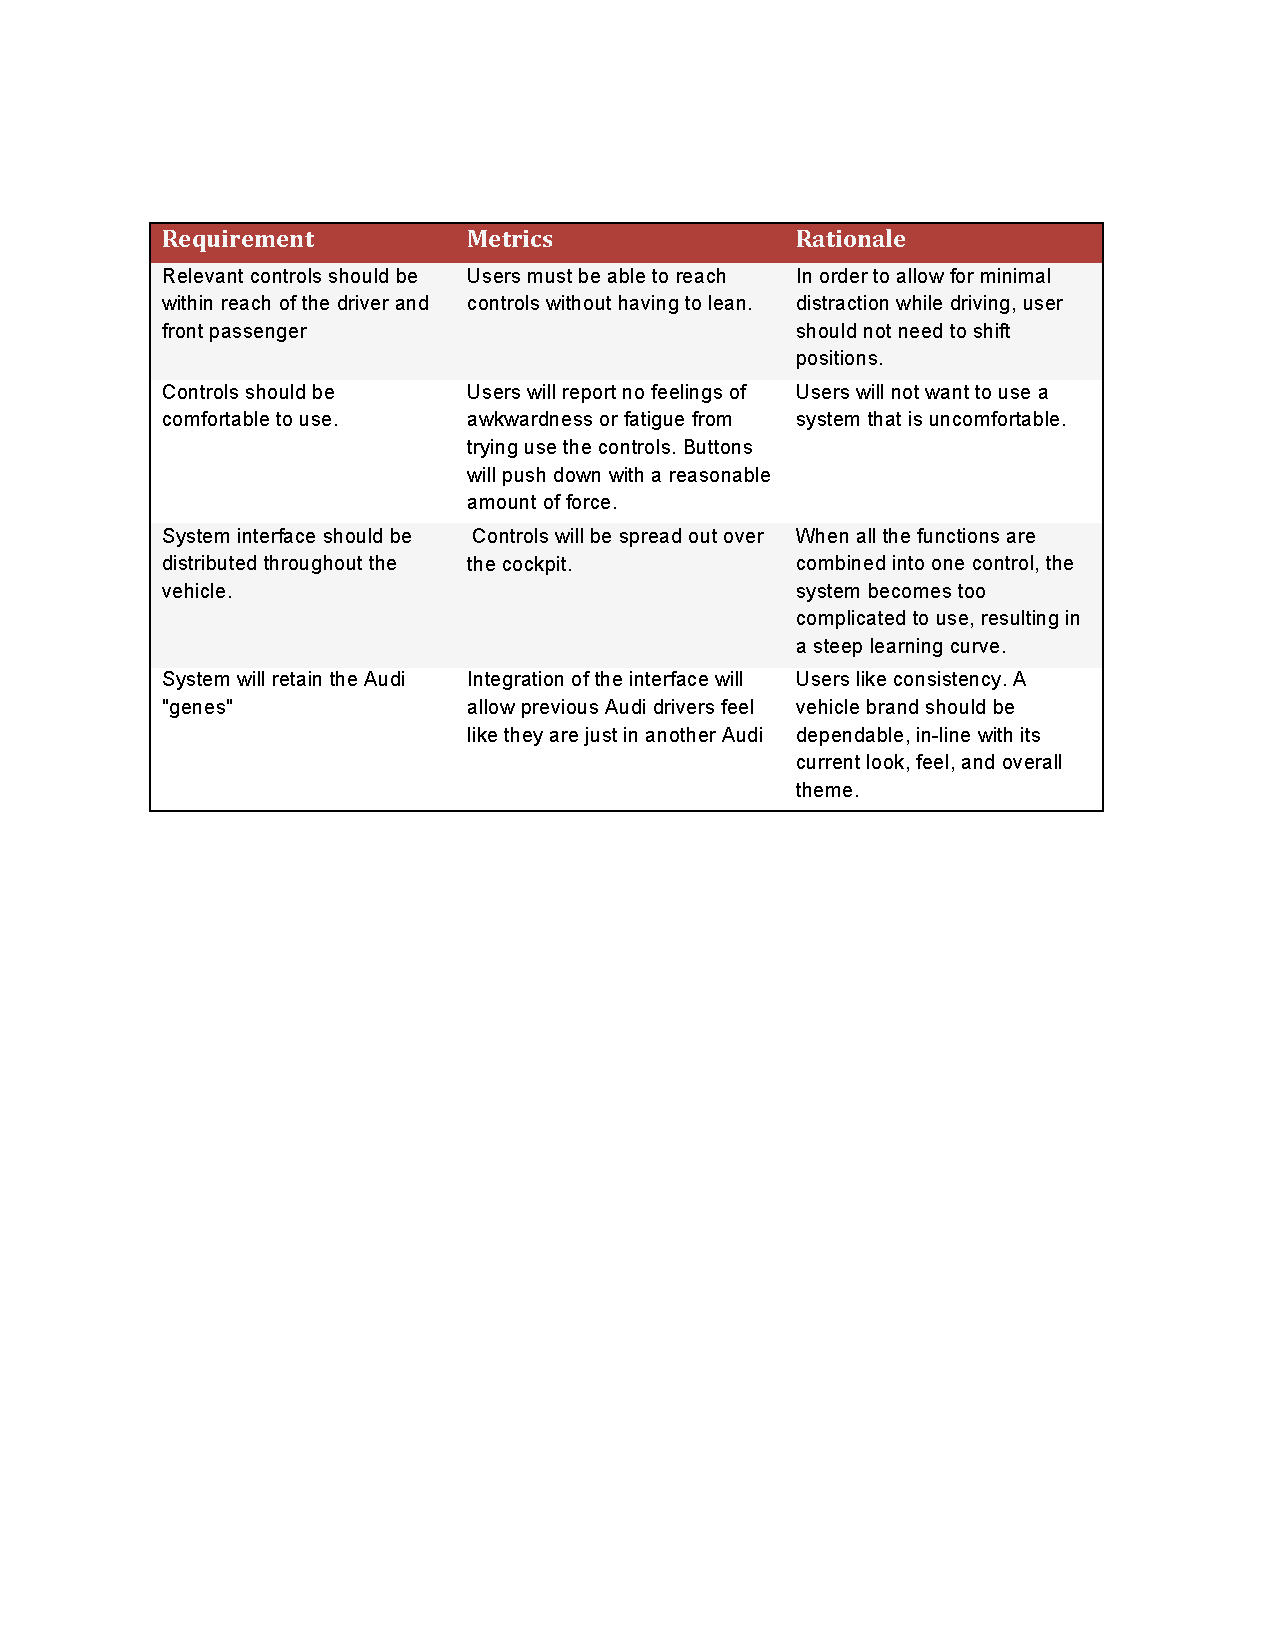
\includegraphics[width=\textwidth]{Figures/Ch3/Audi08PhysReqs.pdf}
        \caption{Physical Requirements from Audi 2008-09}
        \label{tab:physical-requirements}
\end{table}




%%%%%%%%%%%%%%%%%%%%%%%%%%%%%%%%
% Design Development 
\chapter{Design Development}
\label{sec-development}

\begin{remark}  \color{blue}
\begin{itemize}\tightlist
\item The design is the protagonist of the story; the design team is only a supporting character. 
\item Focus on results (e.g., key findings, insights, lessons learned), not activity (``We brainstormed extensively and eventually settled on two alternative concepts.'')
\item Use lots of images, and not just photographs: diagrams, schematics, flow charts, CAD renderings, etc. are often much more informative than a photo. In any case, use labels pointing to the features you want the reader to appreciate.
\item Lengthy details (e.g. detailed results of technical benchmarking) should go in an Appendix section, with an explicit forward reference from this section.
\item Be professional: for benchmarking, it's essential to properly cite sources of information and provide credits for any images you are using that you did not generate yourselves.
\item Don't refrain from describing ideas that were briefly pursued and dropped. Explain why they were abandoned. In other circumstances they might be worth picking up again.
\item You can use tools such as Pugh concept selection, function-structure diagrams and design decomposition to organize and clarify your design process \cite{Otto07,OttoWood01,UlrichEppinger95}.
\end{itemize}
\normalcolor 

The remaining text in this section contains of excerpts from the Autodesk 2007-08 Fall document \cite{Autodesk2008Fall}.
\end{remark}

The broad scope of our problem statement allowed the team members to use their imaginations and arrive at creative solutions. We drew from our diverse individual experiences to redefine the problem as we learned more about existing collaborative tools and practices. Throughout the design development process we balanced pushing forward with our current ideas while constantly looking for new directions. 

\begin{figure}[h]
	\begin{center}
		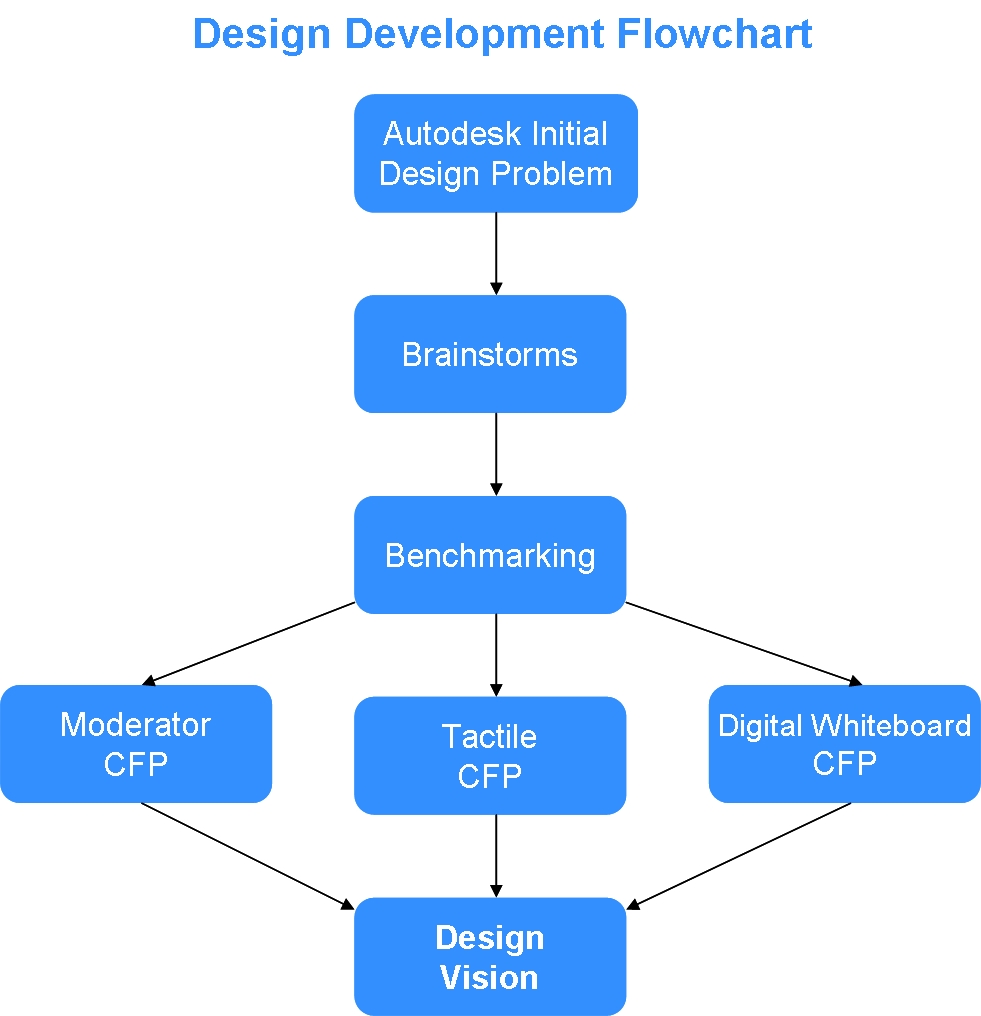
\includegraphics[keepaspectratio, width=4in]{Figures/Ch4/Design_Development_Flowchart.jpg}
	\caption{The design team's development process.}
	\end{center}
	\label{fig:Design_Development_Flowchart}
\end{figure}

\section{Brainstorming}
\label{sec:brainstorm}

	Our experience in brainstorming was unique in that we were observing and studying our own behavior while exploring solutions. We were constantly studying our own triumphs and shortcomings in the hopes of gaining insight into team dynamics. The results of our multiple brainstorms throughout the fall quarter can be into categorized the following categories:

\subsection{Communication}

\begin{figure}[h] 
	\begin{center}
		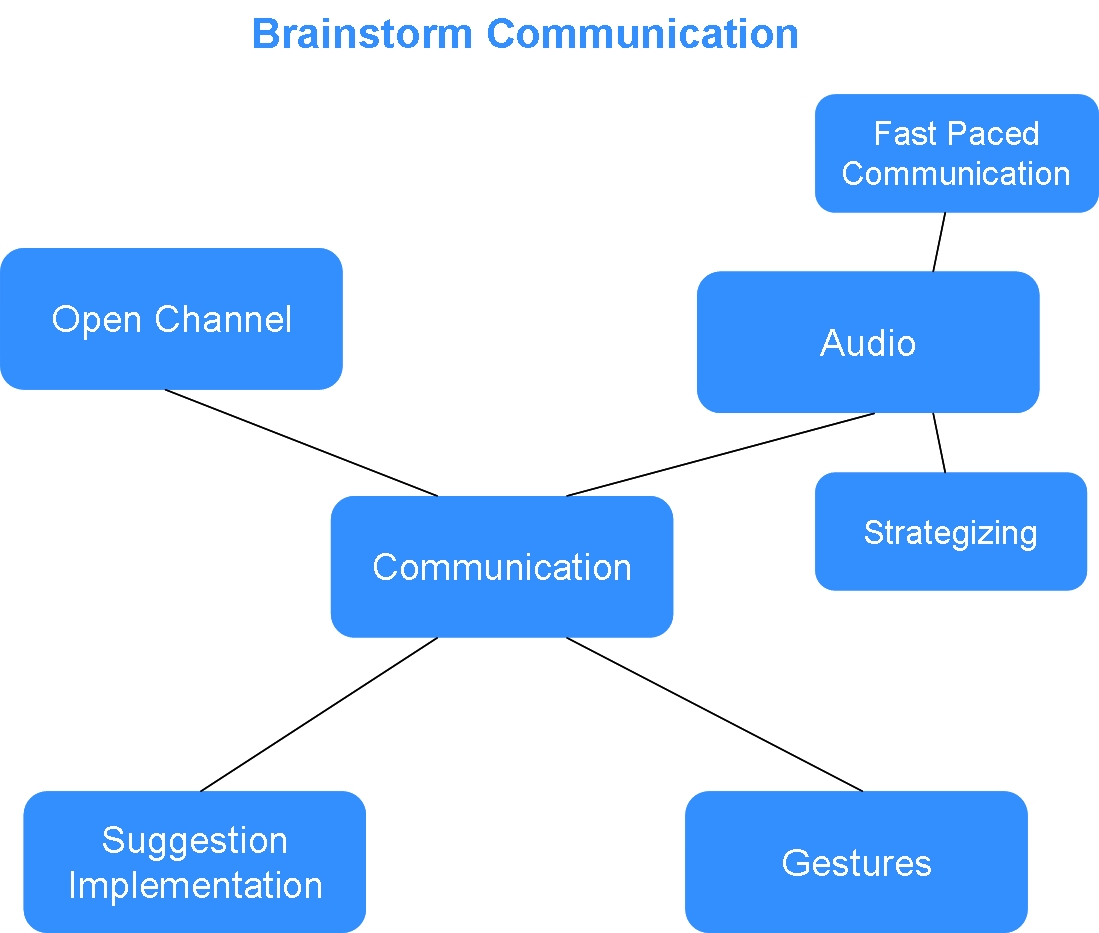
\includegraphics[keepaspectratio, width=3in]{Figures/Ch4/Brainstorm_Communication.jpg}
	\caption{Key components of communication in design meetings}
	\label{fig:Brainstorm_Communication}
	\end{center}
\end{figure}

\begin{itemize} \tightlist 
\item {Open channels}
\item \begin{itemize} \tightlist Audio and video channels are often inundated with information, even if they are not the most effective means to transmit a piece of information. The team learned that messages are most clearly conveyed when they are free from interference. \end{itemize}
\item Integrate suggestions quickly
\item \begin{itemize} \tightlist People can build onto other's ideas immediately, and rapidly change the direction of the conversation. \end{itemize}
\item \textbf{Verbal communication is the most flexible}
\item \begin{itemize} \tightlist The team learned from their experience playing cutting-edge multiplayer videogames that verbal communication was the most relied upon medium during fast and slow paced activities. It's versatility and low-bandwidth warranted future attention. \end{itemize}
\item Gesture
\item \begin{itemize} \tightlist Gesture is frequently used when explaining an idea. Often, the drawings produced do not look at all like the concept being developed, but the act of drawing in and of itself can be like a gesture, showing how something will work, or where it will be placed, and so forth. \end{itemize}
\end{itemize}

\begin{center}
\color{blue}
The rest of this subsection is omitted for brevity
\normalcolor
\end{center}

Some key realizations from the brainstorming phase were that social factors and communication shortcomings had alot of opportunity for development. We decided to give special attention to social benchmarking in addition to our technological research.

\section{Research and Benchmarking}
	The team's research and benchmarking efforts were focused on three major categories: human-machine interfaces and input devices, social dynamics, and communication. The methods the team utilized to research items in these three main categories  included trying out hardware, drawing on previous experience, participating in improv exercises, researching existing solutions, and speaking to experts from design, neuroscience, and computer science.
	
\subsection{The Nintendo Wii \textregistered - Accelerometer-based input)}

\begin{figure}[h] 
\centering
		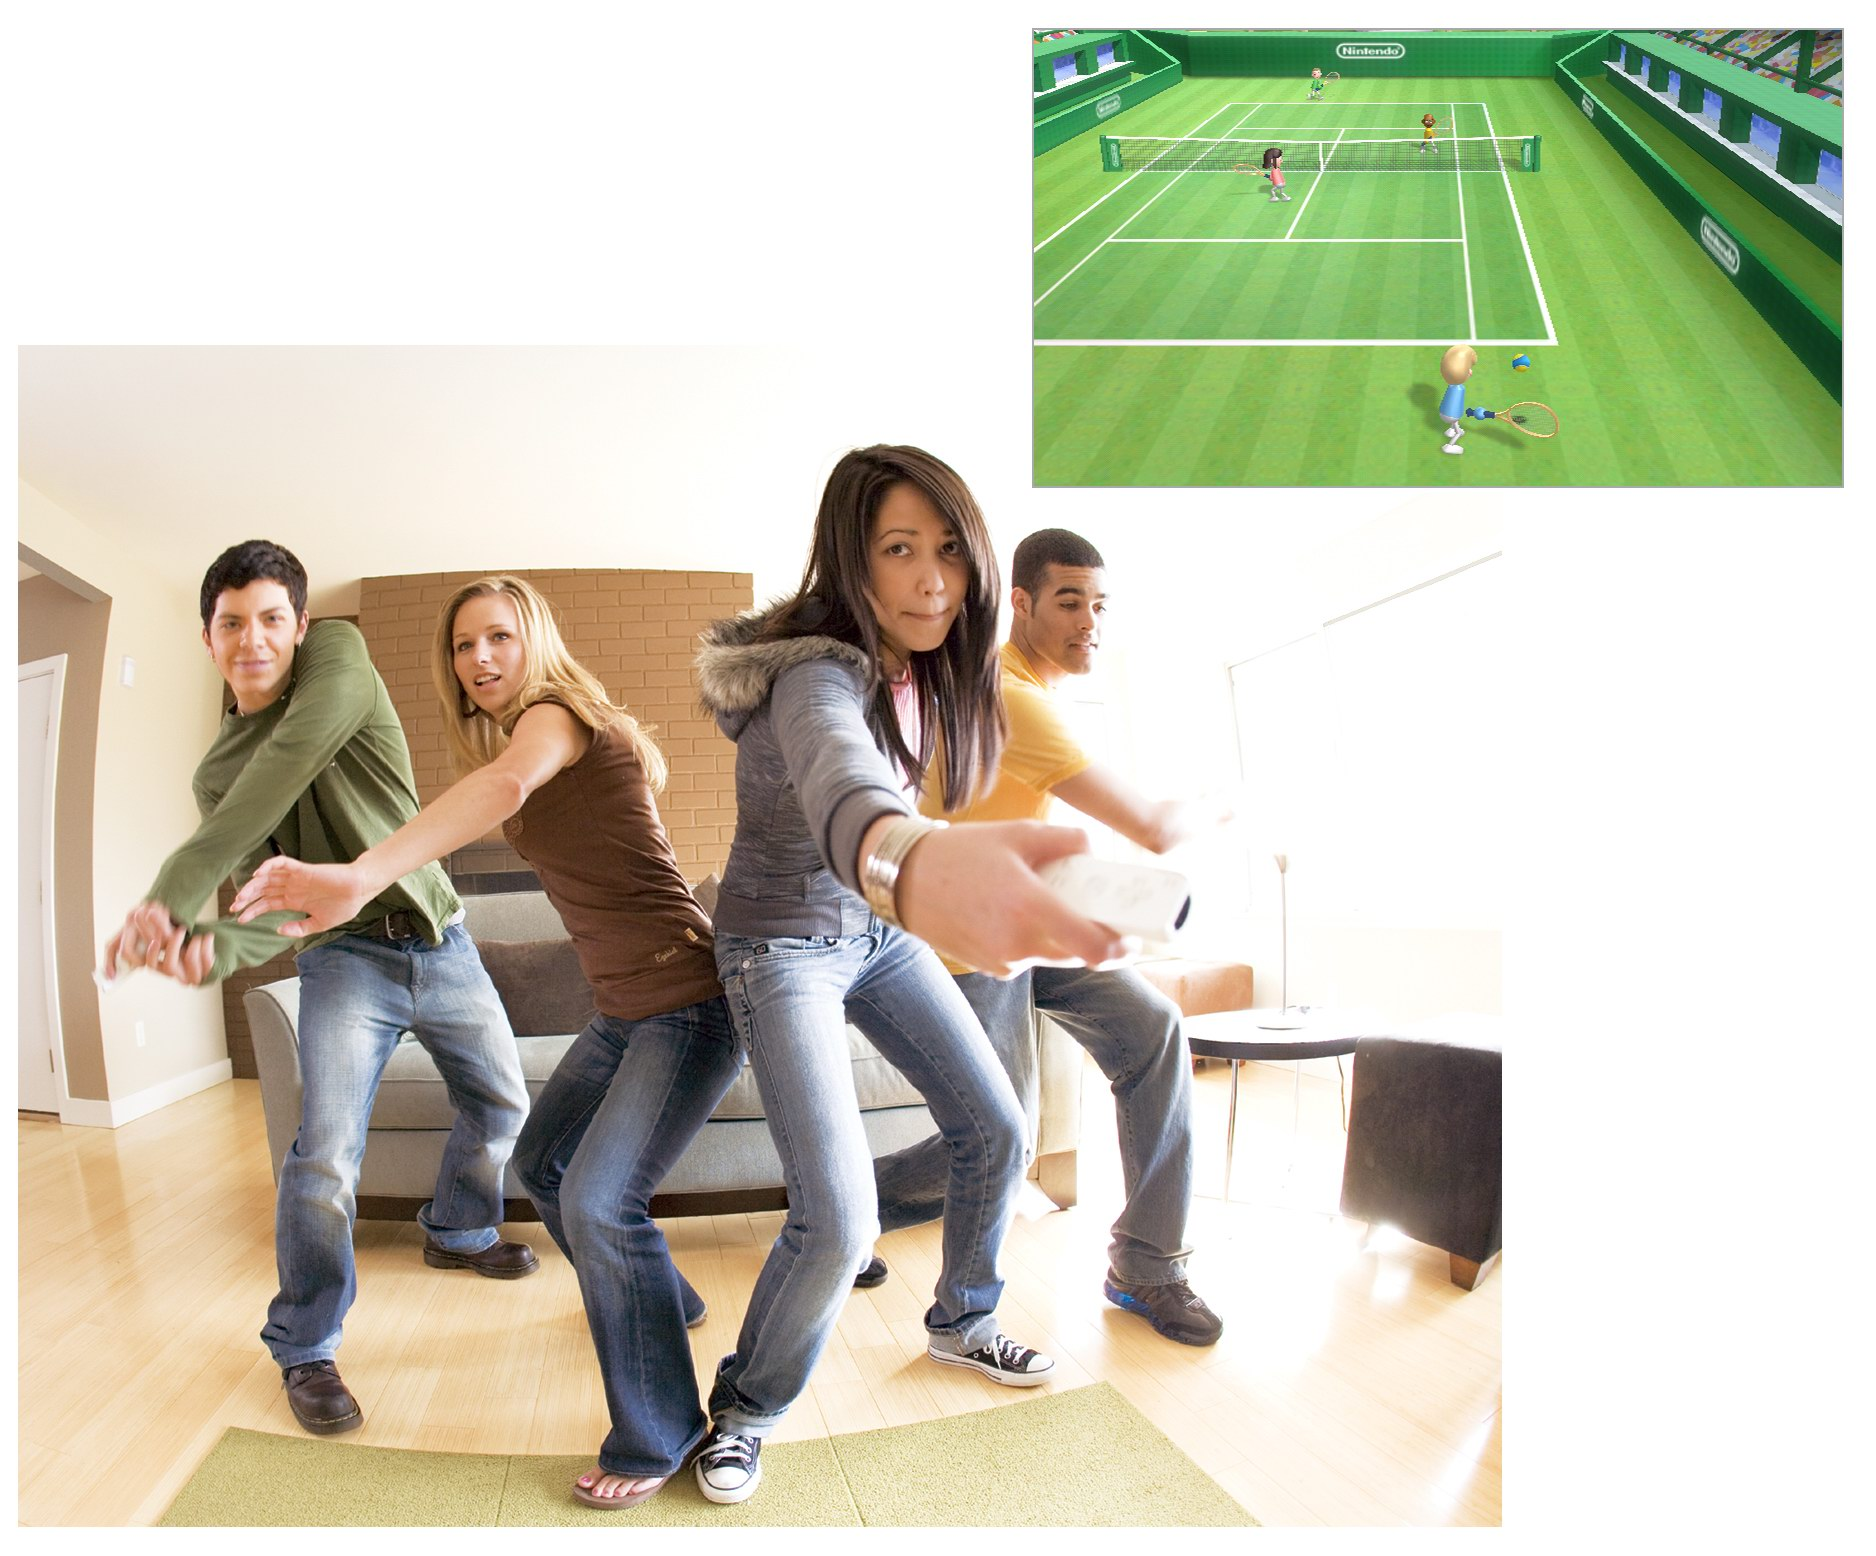
\includegraphics[keepaspectratio, width=4in]{Figures/Ch4/Wii.jpg}
%Note the use of a short caption tag for the list of figures.
	\caption[Nintento Wii]{People playing Wii Sports on the the Nintendo Wii \textregistered.
	\color{blue}Ideally there would be a citation to the URL this photo came from\normalcolor. }
\end{figure}

	The team investigated some unconventional means for data input. Gesture-based input devices like the Nintendo Wii controller offer the possibility of an intuitive, and compelling way to interact with someone at distance via digital means.  For navigating through Windows or other applications, the team found the Wii to be  more challenging than a conventional mouse.  Accelerometers are adept at capturing large motions rather than precision pointing and would need to be utilized as such. Potential applications could be for interfacing with avatars or tactile feedback systems. The Wii controller could be used as a gesture-based communication device to control a personal avatar or send and receive tactile messages.
	
\noindent \textbf {Key lessons learned}
\begin{itemize} \tightlist 
\item Accelerometer based input devices could be used in gesture-based or tactile communication, but do not fare well in precision pointing.
\item Gesture-based interfaces generate excitement. People want to use input devices that respond to gesture. 
\end{itemize}

\subsection{CyberGlove \textregistered}

\begin{figure}[h] 
\centering
		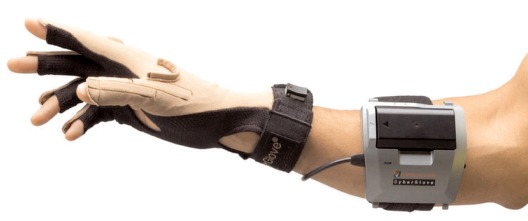
\includegraphics[keepaspectratio, width=4in]{Figures/Ch4/CyberGlove.jpg}	
%Note the use of a short caption tag for the list of figures.
	\caption[Cyberglove]{CyberGlove \textregistered gesture-based input device. \color{blue}Ideally there would be a citation to the URL this photo came from\normalcolor.}
\end{figure}

\begin{center}
\color{blue}
The rest of this subsection is omitted for brevity
\normalcolor
\end{center}

\subsection{EEG and Participation Monitor}

\begin{figure}[h] 
\centering
		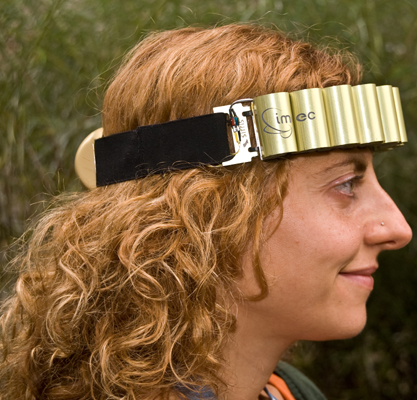
\includegraphics[keepaspectratio, width=3in]{Figures/Ch4/EEG.jpg}
	\caption[Wireless EEG]{Example of the first available wireless EEG tool, made by IMEC. \color{blue}Ideally there would be a citation to the URL this photo came from\normalcolor.}
\end{figure}

	The team met with Alicia Warlick, a researcher in the Stanford Neuroscience Department, and her research in monitoring brainwaves. We discussed the possibility of monitoring whether meeting participants were actively paying attention by using an EEG. This is a method for measuring the activity level of the brain. There is opportunity to use this as a metric for testing our final product, or potentially in the product itself as a means to collect data on user participation level.

\noindent \textbf{Key lesson learned}
\begin{itemize} \tightlist
\item  Electrodes could be placed on the users forehead and scalp to measure EEG readings, which conveys information about whether someone is engaged in what they are doing, or if they are withdrawn.
\end{itemize}

\begin{center}
\color{blue}
The rest of this subsection is omitted for brevity
\normalcolor
\end{center}

\section{Critical Function Prototypes (CFP)}
	The initial benchmarking phase lead the team to realize that there were three major challenges to solve: bridging the proximity gap, moderating brainstorming, and conveying and recording ideas. The team decided to tackle all three of these major challenges and designed four CFPs in an attempt to solve, or at least start answering some of, the questions these challenges brought up. 

\subsection{Tactile CFP}
	
\subsubsection{Tactile CFP Concept Development}

The team wanted to come up with a creative solution that would enhance distance communication. Although we identified software having an important role in our solution, we wanted to try to design something physical. We had to answer these questions that were raised after the benchmarking process:
\begin{itemize} \tightlist
\item How can we simulate proximity for remote meetings?
\item How can we implement action-event control?
\item What senses can we stimulate that aren't normally used?
\item What is a low bandwidth solution?
\end{itemize}

	The team decided that building a tactile messaging system would solve all four of the aforementioned questions. Tactile messages could replace common interpersonal interaction found in same room meetings. It is normal to welcome each other with a  handshake, make eye contact throughout a meeting, smile at each other, and give high-fives to congratulate others. These occurrences are all absent from distance meetings. A tactile message corresponding to each of these gestures would allow users similar opportunity to communicate as if they were sharing the same physical meeting room.
	
	The team learned that immersive activities like videogames take advantage of action-event control to offer users a seamless means to interact with their environment. A tactile message could quickly be sent over an open channel and pressing the �on� button would instantly message the recipient.
	
	Out of the five senses (sight, hearing, taste, touch, and smell), sight and hearing are the most relied upon during meetings. The team considered possibilities in taste and smell messaging but continued with touch, since delivery of tactile messaging was much more straightforward. Since conventional distance meetings only send and receive auditory and visual information, tactile messages would be distinct and easy to identify. The team believed that tactile messages (high, low, or off) would be low bandwidth.

	\begin{figure}[h] 
\centering
		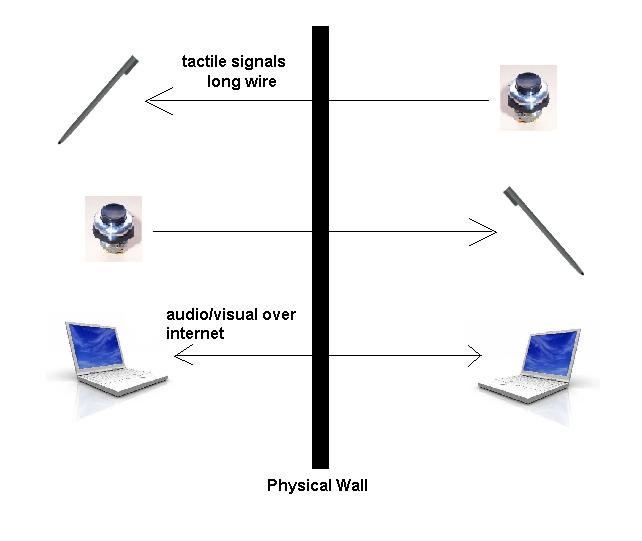
\includegraphics[keepaspectratio, width=4in]{Figures/Ch4/tactileCFPschematic.jpg}
	\caption{The team's whiteboard during a brainstorm session}
\end{figure}

	The team wanted to test the effectiveness of tactile messaging and decided against a TCP/IP protocol that sent messages between Stanford and PUJ. The code to write such a protocol was extant and it was unnecessary to include it in our prototype. The team simplified the setup and created two stations separated by physical barriers (a wall and 50' of distance), to simulate a distance meeting. Each station would have a vibrating tactile device for each seated participant at that station and a high/low button assembly to activate the vibrating tactile device for each participant at the other station. Initially the devices were supposed to operate as ''on'' or ''off.'' The team decided that having more variability in the operating speeds of the motors would increase the number of different messages that could be sent, and added a high and low voltage button (1.2V and 0.6V).
	We were curious to see if effective communication could take place if a distant colleague could see what sketches his distant colleague was drawing. To test this, we used webcams to send live video of what the participants drew on their drawing pads to the other stations.

\subsubsection{What is critical about this CFP?}
	The team identified these questions as critical before testing:
\begin{enumerate} \tightlist
\item Can it create immersion?
\item Does it improve upon existing communication tools?
\item Is it easy to understand?
\item Is it intuitive?
\item When should it be used?
\end{enumerate}

\begin{figure}[h] 
	\begin{center}
		\includegraphics[width=3in]{Figures/Ch4/tactile_seating.jpg}
	\caption{The orientation of the two tactile messaging stations.}
	\end{center}
\end{figure}

%A transcript of the meeting with tactile feedback is available in Appendix \ref{sec:tactiletranscript}.

\subsubsection{Lessons Learned}

	Tactile sensation is an effective means of communicating contextual information. The messaging system delivered instant vibration between the two stations, helping preserve the flow of conversation without impeding it. Using the vibrations to alert the other users that you wanted to say something was a good way to make comments at the precise time you intended. The tactile devices were \textbf{easy to use} and the participants were encouraged to use them as they saw fit. We noticed that \textbf{vibrations were used most frequently to add emphasis} � to accompany laughter, to confirm agreement, offer praise for a good idea � and to interrupt the speaker. Interruptions consisted of calls for clarification on a point raised or disagreement with an opinion. Interrupting someone who is speaking can cause the speaker to lose his train of thought or become otherwise agitated. We noticed that \textbf{users preferred to send low speed vibrations} as a gentle interruption as a first attempt to get the speaker's attention. If the first few low speed vibrations did not stop the speaker, the high speed vibrations could be sent, and these usually registered right away. We observed that users reserved high speed vibrations for urgent or important messages. 
	
	
	The signals were mostly easy to detect, but it was \textbf{not always clear what those signals were trying to communicate}. Ambiguous or superfluous signals distracted the receiving user from the meeting and the confused user would ask, ''Did you just buzz me?'' or ''�Why did you buzz me?'' These confused questions would stall the meeting for everyone until the sender was revealed and was able to explain what they were trying to communicate. 
	
	Vibrations, however, were easily detectable despite loud side conversations, a party in a neighboring room, and constant distractions from people walking by. We attribute this to the fact that the tactile channel is uncrowded compared to the audio channel. In a loud environment it is difficult to pick out audio communication from Skype. Visual distractions make it difficult to focus on the laptop monitor. The tactile sensation rarely stimulated in a teleconference, thus making the slightest vibration very noticeable. 
	
	We tried two different vibrating interfaces, a vibrating pen and a vibrating wrist patch. The wrist patch was unanimously rejected by the participants because 1) the double stick tape that connected the patch to the user's skin was either too sticky and removed arm hair or not sticky enough after a few uses and would fall off, 2) was tethered to the power supply and restricted movement to the point where the hand with the patch was essentially stationary, 3) vibrations on your wrist are not comfortable, and 4) worry that the patch might give the user an electrical shock. The pen had a practical use, writing, and although the pen was connected to the power supply, the user was not, and the range of motion was adequate enough to write anywhere on the drawing space.
	
	We finally compared the tactile messaging conference to previous experiences with video conferencing and audio conferencing. These results are summarized in Appendix \ref{sec:Appendix1}.
	
		\begin{figure}[h] 
\centering
		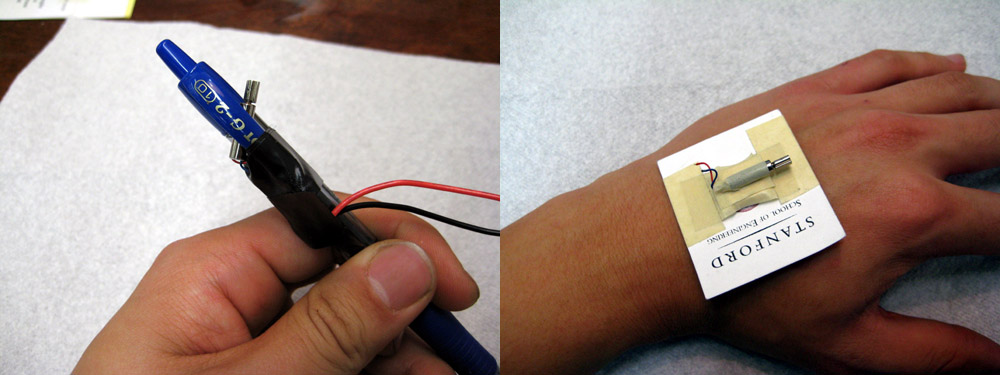
\includegraphics[width=0.8\textwidth]{Figures/Ch4/tactile_motor.jpg}
	\caption[Messaging station wires]{The orientation of the two tactile messaging stations. (Note: the wires connecting the patch to power supply are not in this photo)}
\end{figure}

	The tactile messaging critical function prototype was a success in that it definitively answered all the critical questions we asked ourselves before testing.

%%%%%%%%%%%%%%%%%%%%%%%%%%%%%%%%
\chapter{Design Description}
\label{design-description}

\begin{remark}\color{blue}
The description section defines what the design is. If you find yourself adding rationale, or discussing design alternatives, you are writing text that should be moved into the Development section. A few teams find that this section fits more naturally if it comes before the Design Development section.

In the Fall quarter, the design will be in an early stage and this section is largely a proposal for what the design should be (you can call it that, explicitly). Even so, on the basis of preliminary need-finding, benchmarking and critical function evaluation, you have some idea of what is appropriate. Take a point of view and assert it. A CAD model or systems diagram of a concept may be appropriate.
\normalcolor \end{remark}

\section{Vision}
\label{vision}

\begin{remark}\color{blue}
Use this section to describe your vision or proposal for what you think the design might be. Ideally you should have a sketch, a diagram or other images to help define it.
\normalcolor\end{remark}

The remaining text in this section contains of excerpts from the Autodesk 2007-08 Fall document \cite{Autodesk2008Fall}.

\section{Tactile Messaging CFP}

The tactile messaging system was comprised of small Jameco vibrating motors (1.3VDC 8,500 RPM) mounted to ball point pens and wrist patches. A simple switchable voltage supply circuit was created to give each vibrating motor a high (1.2V) and low (0.6V) vibrating speed (\ref{fig:tactile_circuit}). Each voltage level was buffered with LM324 opamps, and the circuits were implemented on protoboards. The high and low speeds were selected by switches. 

\begin{figure}[bhtp] 
	\begin{center}
		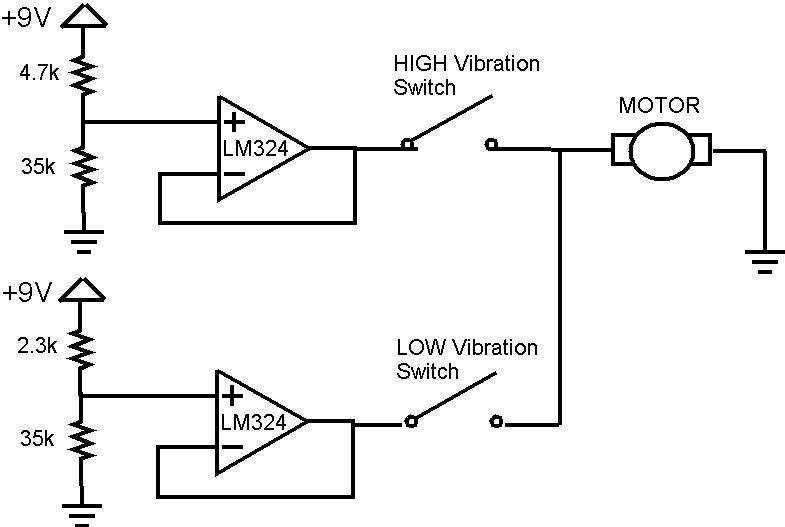
\includegraphics[width= \figwidth]{Figures/Ch5/tactile_circuit.jpg}
	\end{center}
	\caption[voltage divider]{A simple voltage dividing circuit provided 1.2V (HIGH) and 0.6V (LOW) buffered output voltages for the vibrating motor. Switches triggered the high and low voltages. }
	\label{fig:tactile_circuit}  
\end{figure}

\begin{center}
\color{blue}
(Text omitted for brevity)
\normalcolor
\end{center}

Four independent circuits were created to provide messaging to two motors on each side. 90' 16-gauge wire was passed between two stations in the meeting setup shown in \ref{fig:tactile_seating}. Power supplies provided the 9V signal on each side.

\begin{figure}[bhtp] 
	\begin{center}
		\includegraphics[width=3in]{Figures/Ch5/tactile_seating.jpg}
	\end{center}
	\caption[test meeting layout]{Layout of seating during test meeting. Two participants met on one side, with the remote user separated by a wall 50 ft away. }
	\label{fig:tactile_seating}  
\end{figure}

In addition to the tactile hardware, Skype was used for video and audio communication. Video was supplied by standard webcams. We mounted the webcams on risers to show video of a sheet of white paper used as the shared drawing space. We chose to focus the video on ideas rather than facial expressions. 


\clearpage
\section{Moderator CFP}

\subsection{Layout}

The participation moderator was created by using pre-made desktop software applications called widgets. The desktop was set to a white image, with personal spaces for each participant mapped off by a black boundary and labelled with the participant name. In each personal space, a unique Yahoo! Widgets timer was placed. Unique timer's were used to foster a sense of identity- when glancing at the moderator, the team members could instantly recognize their widget rather than look for their name. 

\begin{figure}[htbp]
	\centering
		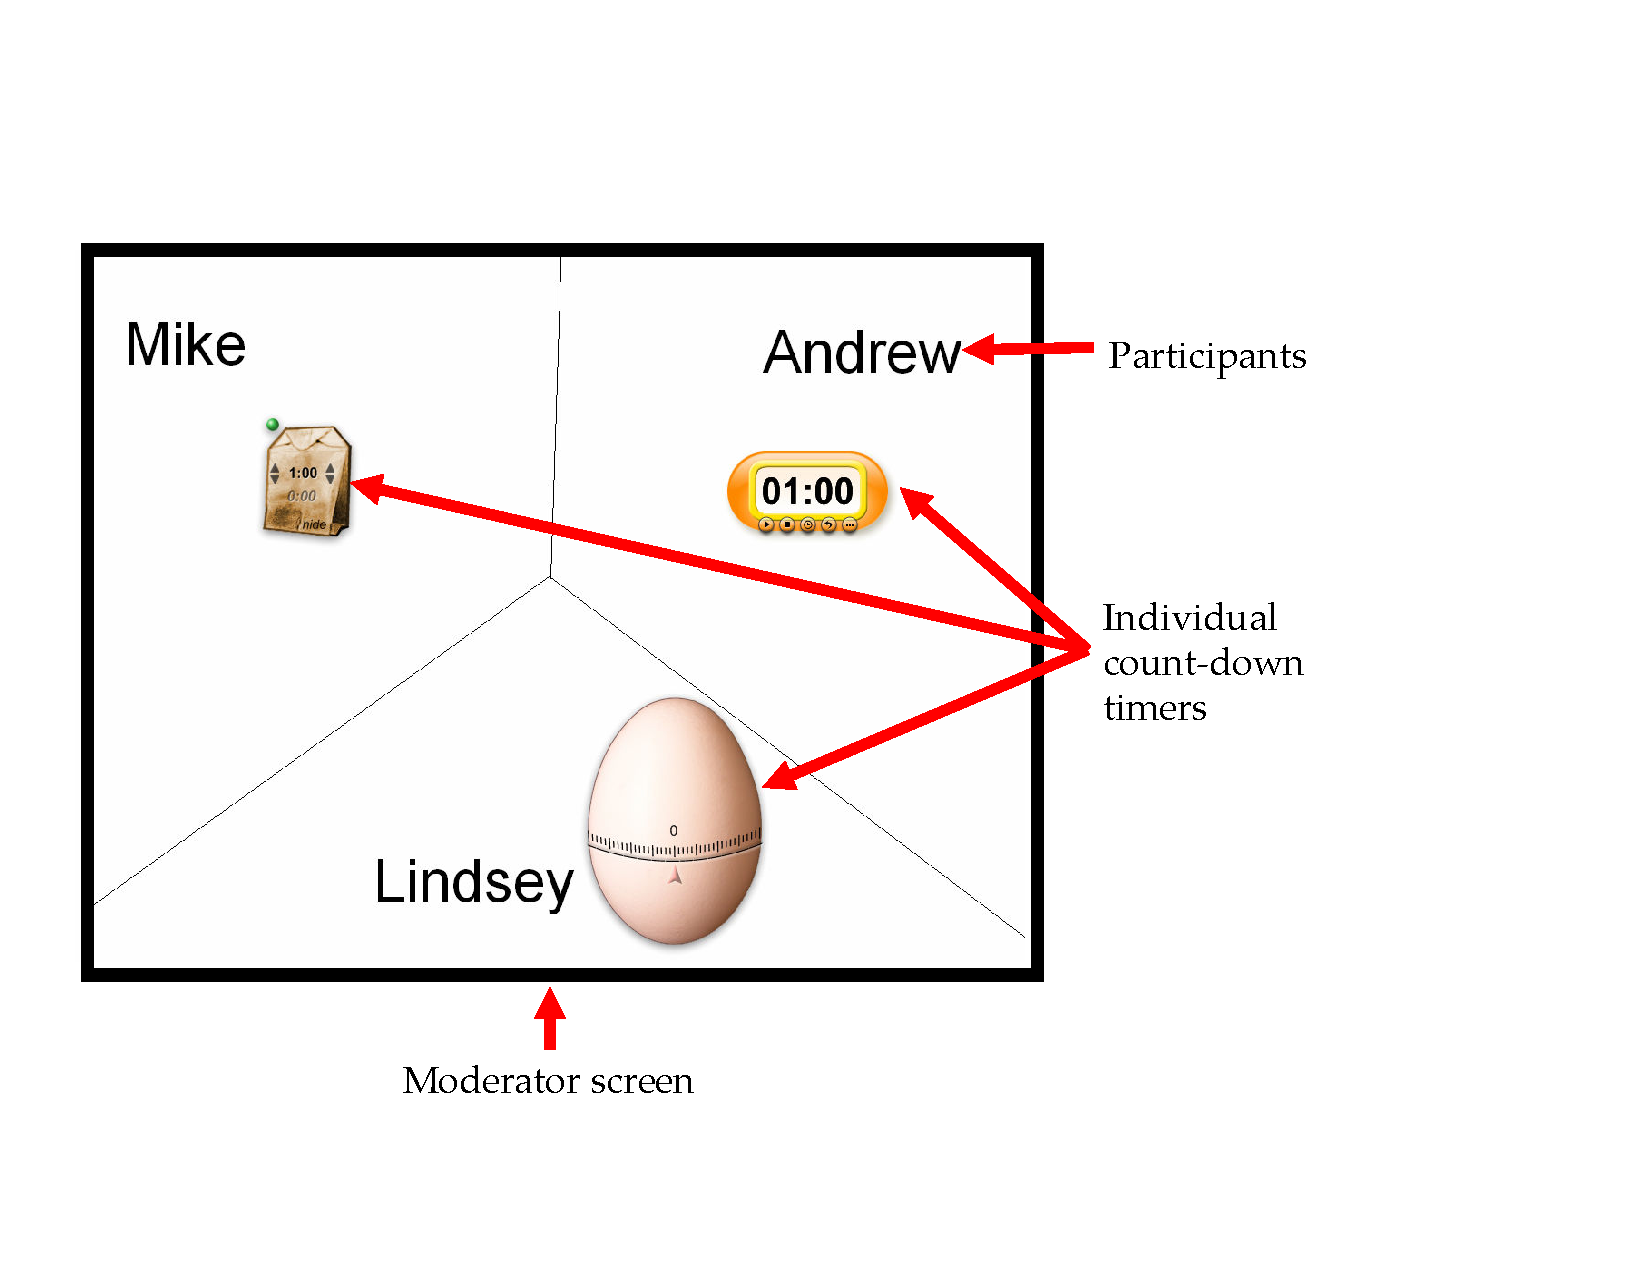
\includegraphics[width=1.00\textwidth]{Figures/Ch5/moderator.pdf}
	\caption{View of moderator display}
	\label{fig:moderator}
\end{figure}

\begin{center}
\color{blue}
(Text omitted for brevity)
\normalcolor
\end{center}


Each was simply a countdown timer with a default starting time, $t_{s}$. As they begin counting down, the amount of time remaining is visible. By clicking twice on any widget, it would reset and begin counting down again from $t_{s}$. The timers were manually reset by one of the teammates during the meeting whenever someone had an interaction. When any timer runs out, it would sound an alarm, designating that the meeting come to a halt until the non-active team member contributes to the conversation. The hypothesis was that, because the timers were visible to the entire team, each member would consciously make an effort to speak before their timer ran out and that no timer would actually buzz, although the rotation of speakers would greatly increase.

The moderator screen was displayed on a 32" LCD display that was positioned 6' from the center of a table where the group met. The layout is detailed in Figure \ref{fig:moderator_setup}. No video or audio conferencing was used -- all team members were local. The objective of the moderator is to support dialogue in meetings, regardless of whether the members are distributed or not. Audio was recorded of each meeting using Cubase software and an IBM laptop's internal microphone, which was placed in the center of the table so each participant could be heard. 

\begin{figure}[h]
	\centering
		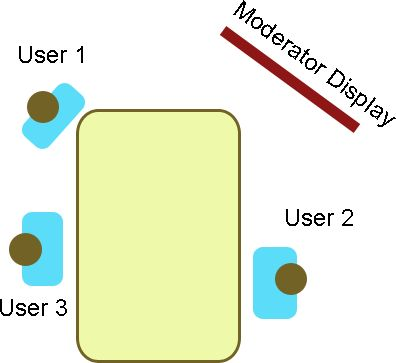
\includegraphics[width=.75\textwidth]{Figures/Ch5/moderator_setup.jpg}
	\caption{Layout of design meeting with moderator prototype}
	\label{fig:moderator_setup}
\end{figure}

\subsection{Procedure}

Three meetings were run to test the moderator. The subject of each was the same - our team brainstormed potential final products knowing the key lessons learned after our benchmarking. Three meetings were run in succession, each lasting 30 minutes. The intention of this was to eliminate any personal changes between meetings. For example, if Mike has a really bad day before coming in for a second meeting, he may be much less talkative than in the previous meeting, but not as a result of the moderator. The first meeting served as the control, and no moderator was used. The two subsequent meetings used the moderator with $t_{s}$ at 2 minutes and 1 minute.

The audio files were analyzed manually by playing back the audio recordings for each meeting and recording the length of each comment that every person made. Fifteen minutes of audio during the middle of each meeting was processed. The data are available in Appendix \ref{sec:Appendix1}. 




%%%%%%%%%%%%%%%%%%%%%%%%%%%%%%%%
\chapter{下学期计划}
\label{project-planning}

\begin{remark}\color{blue}
Teams with global partners face special challenges in  terms of organization, project management and planning.
It is a truism that organizational burden goes as the square of team size. 

To address these issues, we ask each local+global team to prepare a \textbf{plan for Winter quarter} to include in this section. You have just accomplished a first, rough critical function prototype (CFP and CEP) and you have given a presentation and written a document that captures the current state of your vision and findings. You have learned who can do what and how much work it really takes. And you are highly motivated to make Winter go more smoothly and to ``take control'' of your project.
\normalcolor
\end{remark}

% \section{计划交付内容}
% Define briefly what is or will be delivered. A short table with some explanatory text could be used here. Your project plan should include the following non-negotiable items and any sub-tasks or intermediate items'' that lead up to them:

% \begin{itemize} \tightlist
% \item Paper Robot (Jan 11-13) -- a mechatronic warm-up for winter
% \item Dark Horse prototype (Jan 25-27) -- a 2nd CFP that probes the edge of the design space
% \item Travel Docs due (Feb 8)
% \item Funky Prototype (Feb 10) -- a CFP where a potential avenue for the final product is developed
% \item Turning Point presentation (Feb 24)
% \item Functional Prototype Review (March 8-10) -- your latest and greatest as Winter quarter draws to a close. It should give a clear indication of what to confidently expect in June.
% \item Winter Design Documents (March 17)
% \end{itemize}

\section{里程碑}
%When are various elements (e.g., rough prototypes, final prototypes) delivered? When are key tests conducted? These are the dates, times, and places where project progress is observable and/or demonstrated. Again, update with planned versus actual dates as the design progresses.

由于采用增量开发模式去开发一个互联网应用,所以里程碑的概念对我们的意义
并不是很大。尽管如此,开发中还是会有几个需要关注的里程碑:
\begin{itemize}
\item 具备基本功能,完全可上线进行测试的原型---预计在四月完成。
\item 重新设计的机器人外形---预计在四月完成。
\item 丰富并完善过的图形界面,后台经历出错后的系统---预计在五月完成。
\item 针对移动互联网客户端兼容的版本---根据前两个里程碑的实现情况决定
  是否选做。
\end{itemize}

% \section{项目时间线}
% Summarize the projected project time line if it is not already explicit in the project planning representations above.

% Use any of the familiar project development representations including lists, Gantt Charts, Pert Charts (Figure \ref{fig:full-page-example}), bubble diagrams, tables, etc. In addition, you will almost certainly need a list or table of items that says a bit
% more about the items and gives an idea who is going to do what.

% \begin{figure}[bhtp] 
% \centering
%                 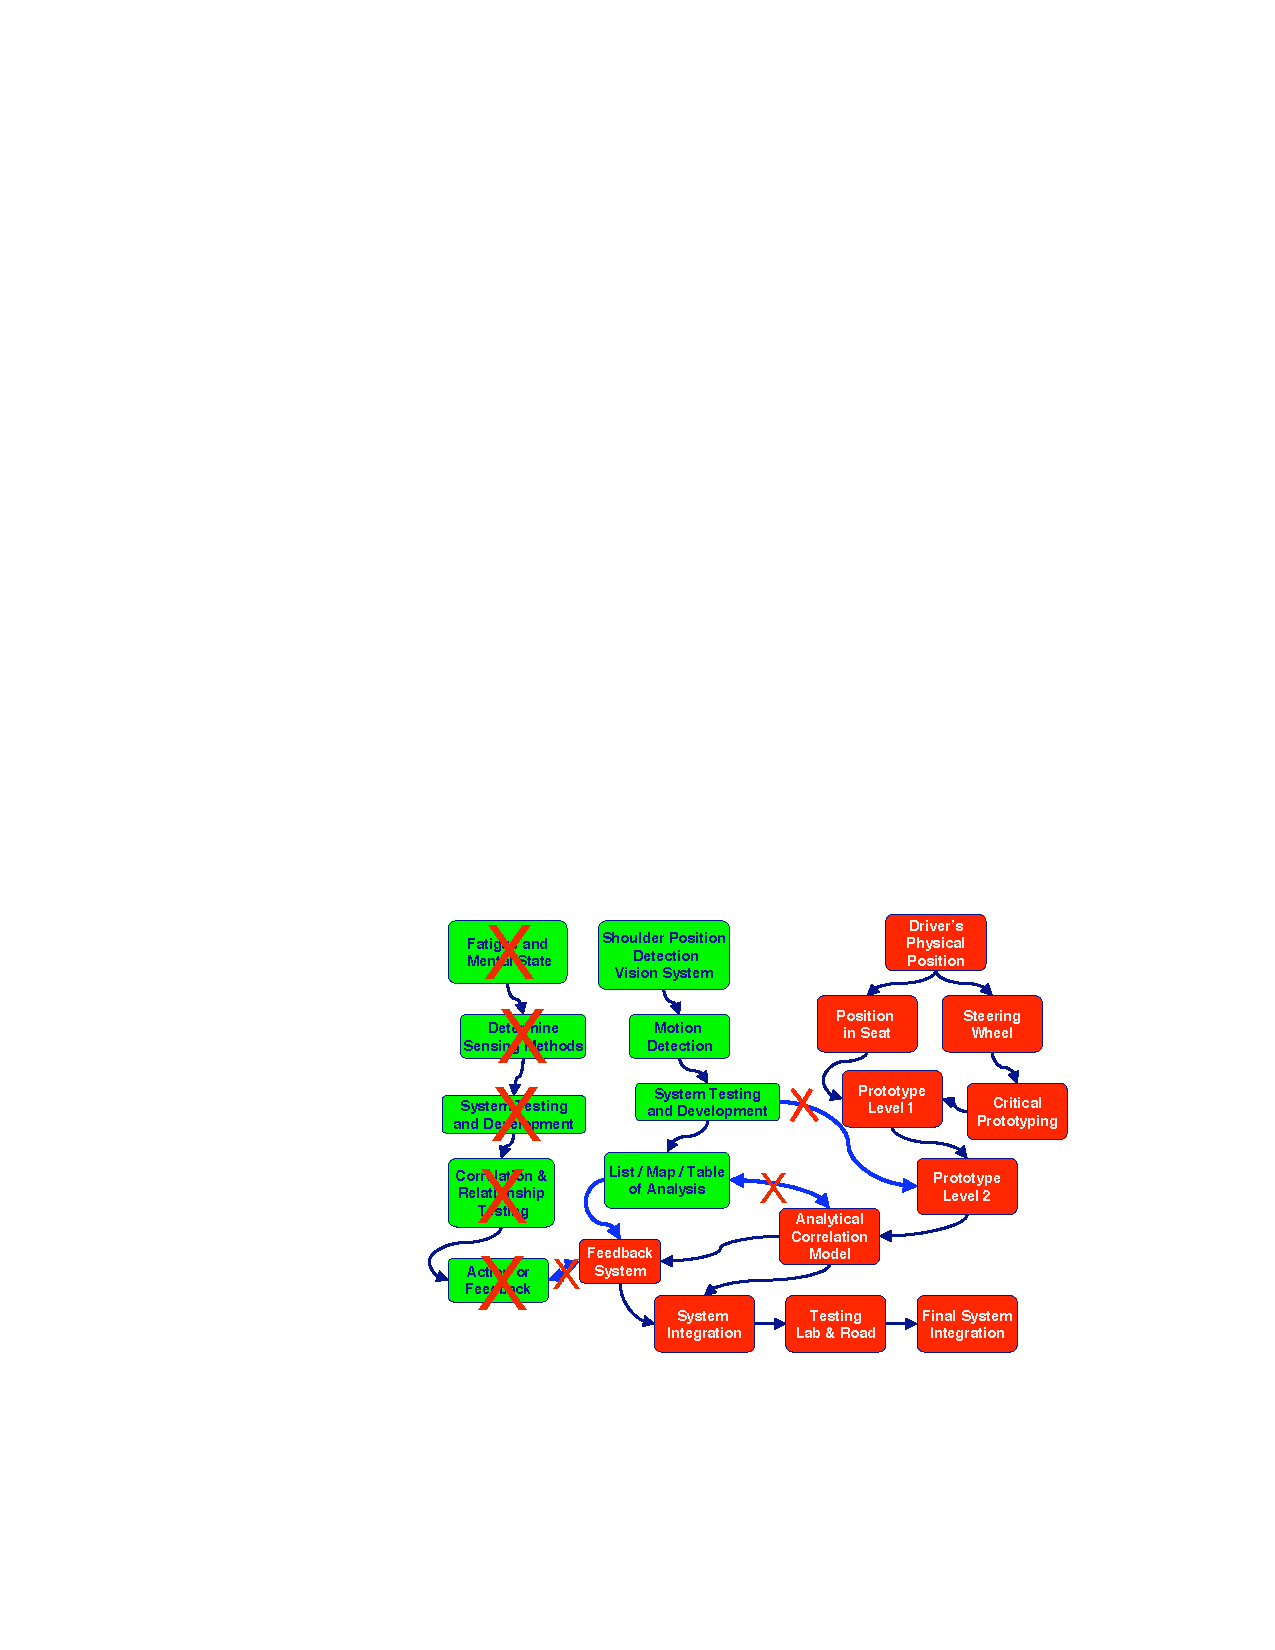
\includegraphics[width=\textwidth]{Figures/Ch6/su-tmit-after.pdf}
%         \caption[Project task replanning example]{In this example from \cite{Toyota01}, Stanford students collaborated with a group at TMIT, Japan. At the end of the Winter quarter it was decided to abandon one branch of the TMIT effort and to eliminate some of the tight coupling that was originally envisioned. }
%         \label{fig:su-tmit}  %Tag for referring to figure in text.
% \end{figure}

% \begin{figure}[p]   % p for "page" for let it be a full page figure!
% \centering
%                 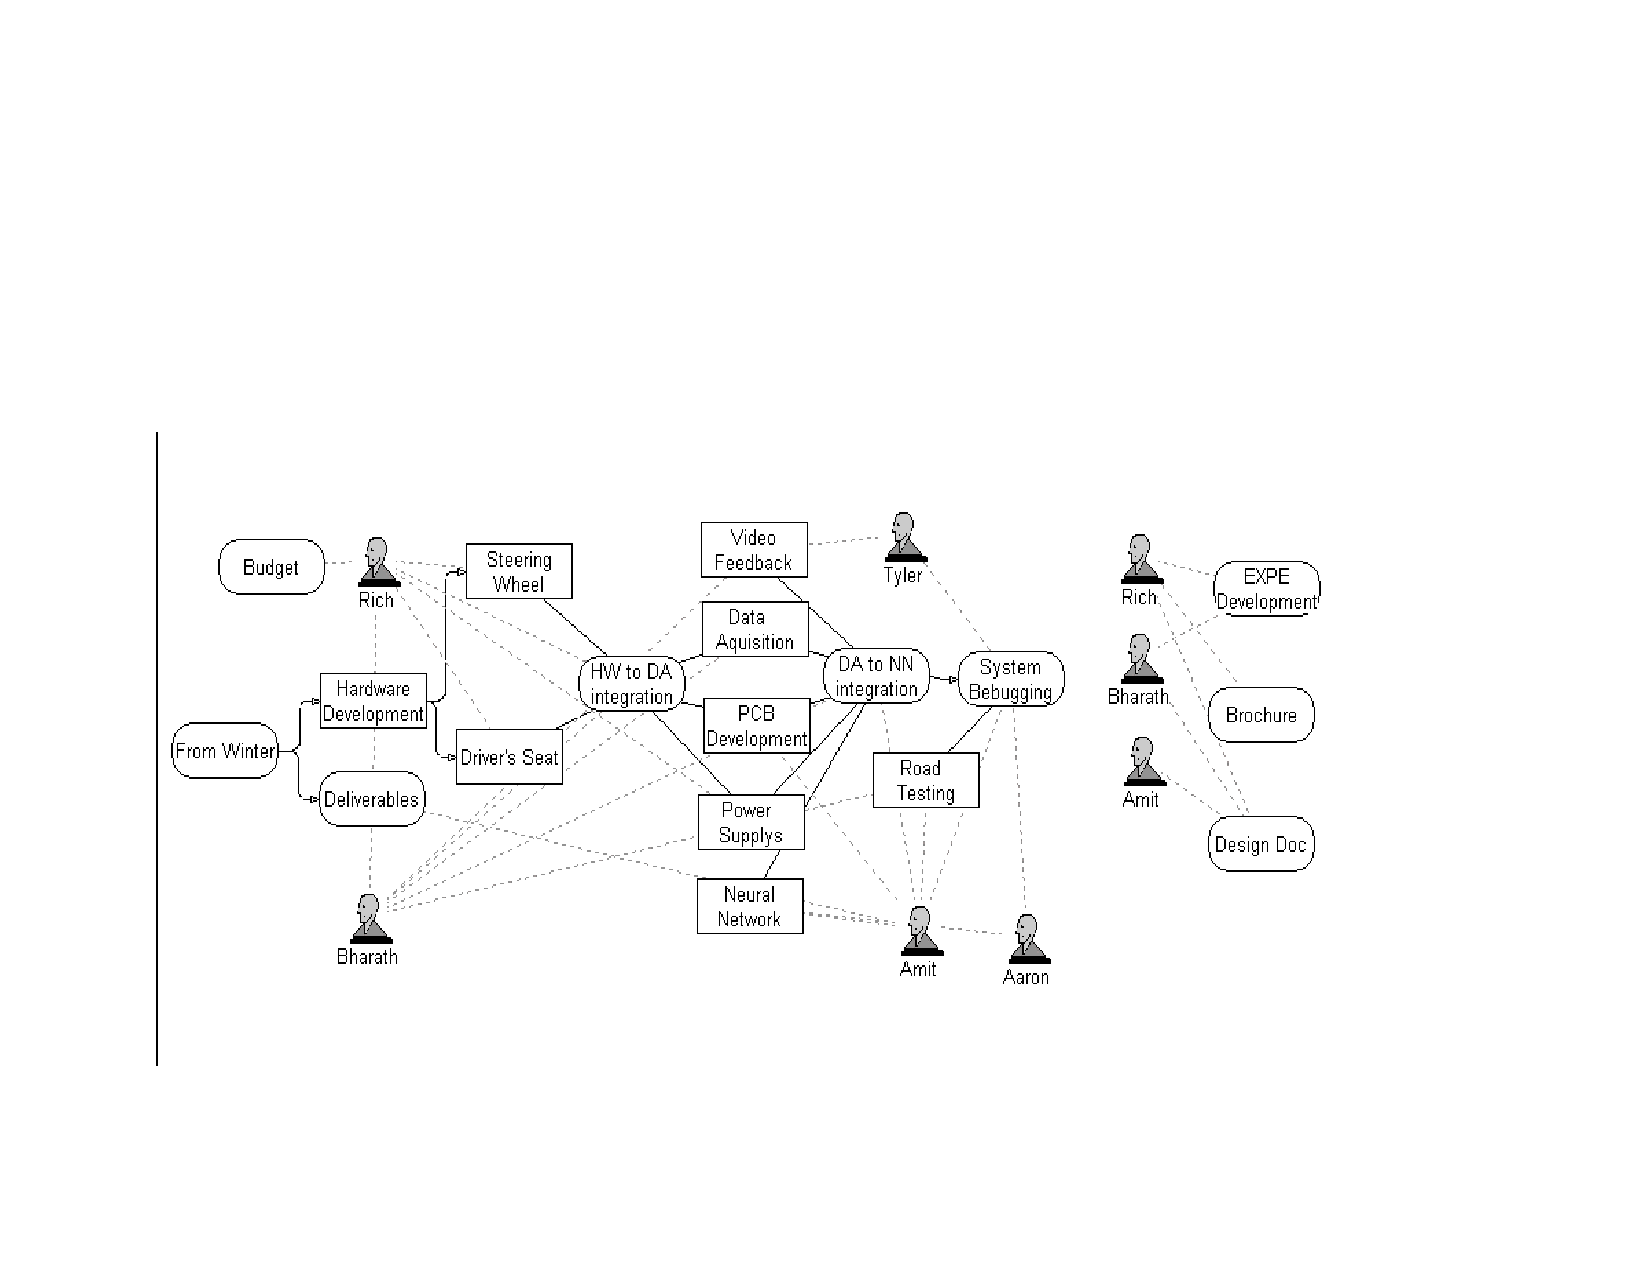
\includegraphics[angle=90, height= 8in]{Figures/Ch6/ideastorm}
%         \caption[Rotated landscape figure example]{An example of taking a large figure and having Latex rotate it 90 degrees to display it in landscape format as a full page figure.}
%         \label{fig:full-page-example}  %Tag for referring to figure in text.
% \end{figure}

\section{项目管理}
%Explain how your distributed and interdisciplinary team will collaborate, communicate and keep itself on-track with respect to the afore-mentioned deliverables.

到目前为止。在项目管理上我们也采取了去中心的分布式的方法。文档系统被部署到网页可访
问的mediawiki上,文件的共享通过匿名ftp实现。下个学期我们计划进一步实现
分布式的项目管理,包括公开的git服务器,提供源代码版本控制和在线浏览;
公开的bugtracker,接受内部和外部的软件缺陷汇报并用于跟踪开发进度。

\section{预算}
%As with any serious proposal, you should include an estimated budget with some specifics about money that has been spent (Fall) and probably will be spent (Winter). Details on vendors can be put in the Appendix.

剩下的预算还很充分,本学期花了800-900¥,由于放弃了购买昂贵的传感器的
计划,所以下个学期的预算比较充足。

\section{思考和目标}
% This is the one section that you would not find in normal research or engineering proposal. But in the spirit that we're doing this in an academic setting, we want to be sure that we reflect on what we're learning and thinking and where we hope to go with it.

% A part of this may include how your team functioned in the fall - explaining how and why your actual design process deviated from what you originally planned, if relevant. (Time lines and milestones often have the look of having been concocted the night before the report is due.)
在本学期的设计中走了一些弯路,比如需求调查做的不充分,CFP的测试不够充
分等。主要原因还是人手不足和时间不够。所以下个学期一定要做好计划,充分
利用好时间。


\chapter{整体框架}

整个系统分为三个部分:受控机器人、用户操作端、服务器。

通信建立流程:服务器在80端口上提供服务,受控机器人访问主页,建立视频广
播信道,随后,远程操作者可进入相同的页面来加入广播信道,从而完成p2p的信
道的建立。此后的视频流等的传输不依赖于服务器的控制。

\section{受控机器人}

上位机即为一台笔记本电脑,下位机为机器人移动的驱动部分。上位机连接服务
器,在后台执行机器人的运动控制程序,收取的移动控制指令通过命名管道发送
到运动控制程序,对于运动的实际控制,使用到了机器人自带的超声波传感器,
因此可以避免一些简单的障碍。显示器主界面显示视频通信页面,接收到的多媒
体信息显示在该页面上,即呈现操作用户方面的音频视频信息。

\section{用户操作端}

呈现给用户的是简洁的网页页面,集成了用户所需的多媒体信息,以及相关的控
制操作实现与帮助提示录像。用户通过“注册—登入—加入已存在的信道“,来完成用户需
要的体验。对于机器人的移动操作通过点击操控按钮或者敲击方向键均可实现。

\section{服务器}

提供常开的固定web服务端口,供用户建立连接。设置并管理用户权限,只有通过注册的用户
才可登录,拥有加入音频视频传输以及控制机器人移动的权限。


\chapter{设计详情及关键实现}

这个系统的特色在于免安装、跨平台、实时性和P2P。

\section{设计特色}

\subsection{免安装}

免安装带来的是用户使用的便捷和免去开发者维护升级的困扰。数据的传输和处
理发生在服务器和浏览器之间,用户只要使用用户名和密码登录,无需下载安装。

另一方面,用户的无需安装也带来了开发者维护升级的方便。我们可以进行小幅
更新而无需发布新的安装包,可以随时修复安全漏洞,也不用同时维护众多版
本——用户使用的版本就是最新的。我们需要做的只是在服务器上部署好,用户需
要做的只是访问我们的主页。

\subsection{跨平台}

随着移动设备狂潮的来临,用户们越来越希望平时享受的服务同样能运行于自己
的移动设备上。另外桌面系统上Windows一家独大的情况不再,Mac用户和Linux
用户的需求日益重要。

借助浏览器这个平台,我们的产品可以实现跨平台化——支持Linux、Android、
Mac OS、Windows等桌面平台和移动平台。可惜的是由于Microsoft和Apple公司
的封闭,目前还无法在iOS和WP平台上使用我们的产品。不过随着时间的推移,
我相信开放的标准必将战胜封闭的平台。

\subsection{实时性}

常见的对Web应用程序的批评是它的相应速度太慢了。确实如此,不过那已经成
为历史了。越来越快的网络带宽和新一代HTML5标准带来的实时性通讯协议
Websocket,带来几乎无延迟的互联网体验。使用我们的系统操纵远程机器人,几
乎感觉不到延迟。

同时新的WebRTC API带来快速、高质量、实时的网络视频的体验。

\subsection{P2P}

没有中央服务器记录您的视频过程,所有的通讯发生于点对点的传输中。这不仅
带来了完全的隐私权和安全性的保证,更带来的是视频会话的快速相应。

\section{关键部分的实现}

运行于服务器端的程序仅仅负责用户的注册、登录,提供静态页面,对控制机器
人的命令的转发。视频通讯发生于用户端的浏览器与机器人端的浏览器之间,完全
没有服务器端的参与。用于控制机器人的程序部署在机器人一方,对用户透明。

\subsection{服务器端}

服务器端使用node.js作为应用服务器。使用express网站框架,采取MVC的设计
模式。使用mongodb存储用户数据。使用socket.io与机器人端进行实时通信。

\subsection{客户端}

网页采用bootstrap进行美化。使用socket.io与服务器进行实时通信,发送对机
器人的控制指令。使用www.freshtilledsoil.com开发的webRTC组件进行实时、
点对点的视频通讯。

\subsection{机器人端}

由于浏览器的沙盒机制,单纯使用网页技术来控制机器人是不切实际的,所以需
要单独的部分来控制机器人。机器人端采用了服务器端相同的node.js进行开发。
为了在任何网络环境中都能够使用,采取主动连接服务器的方式,从而可以在局
域网内正常工作。连接建立后,接受来自服务器转发的来自于用户的控制指令。
随后本部分组件根据接收到的命令控制机器人采取相应动作。


\chapter{实现效果}

机器人外形如下

\begin{figure}[h]
        \centering
                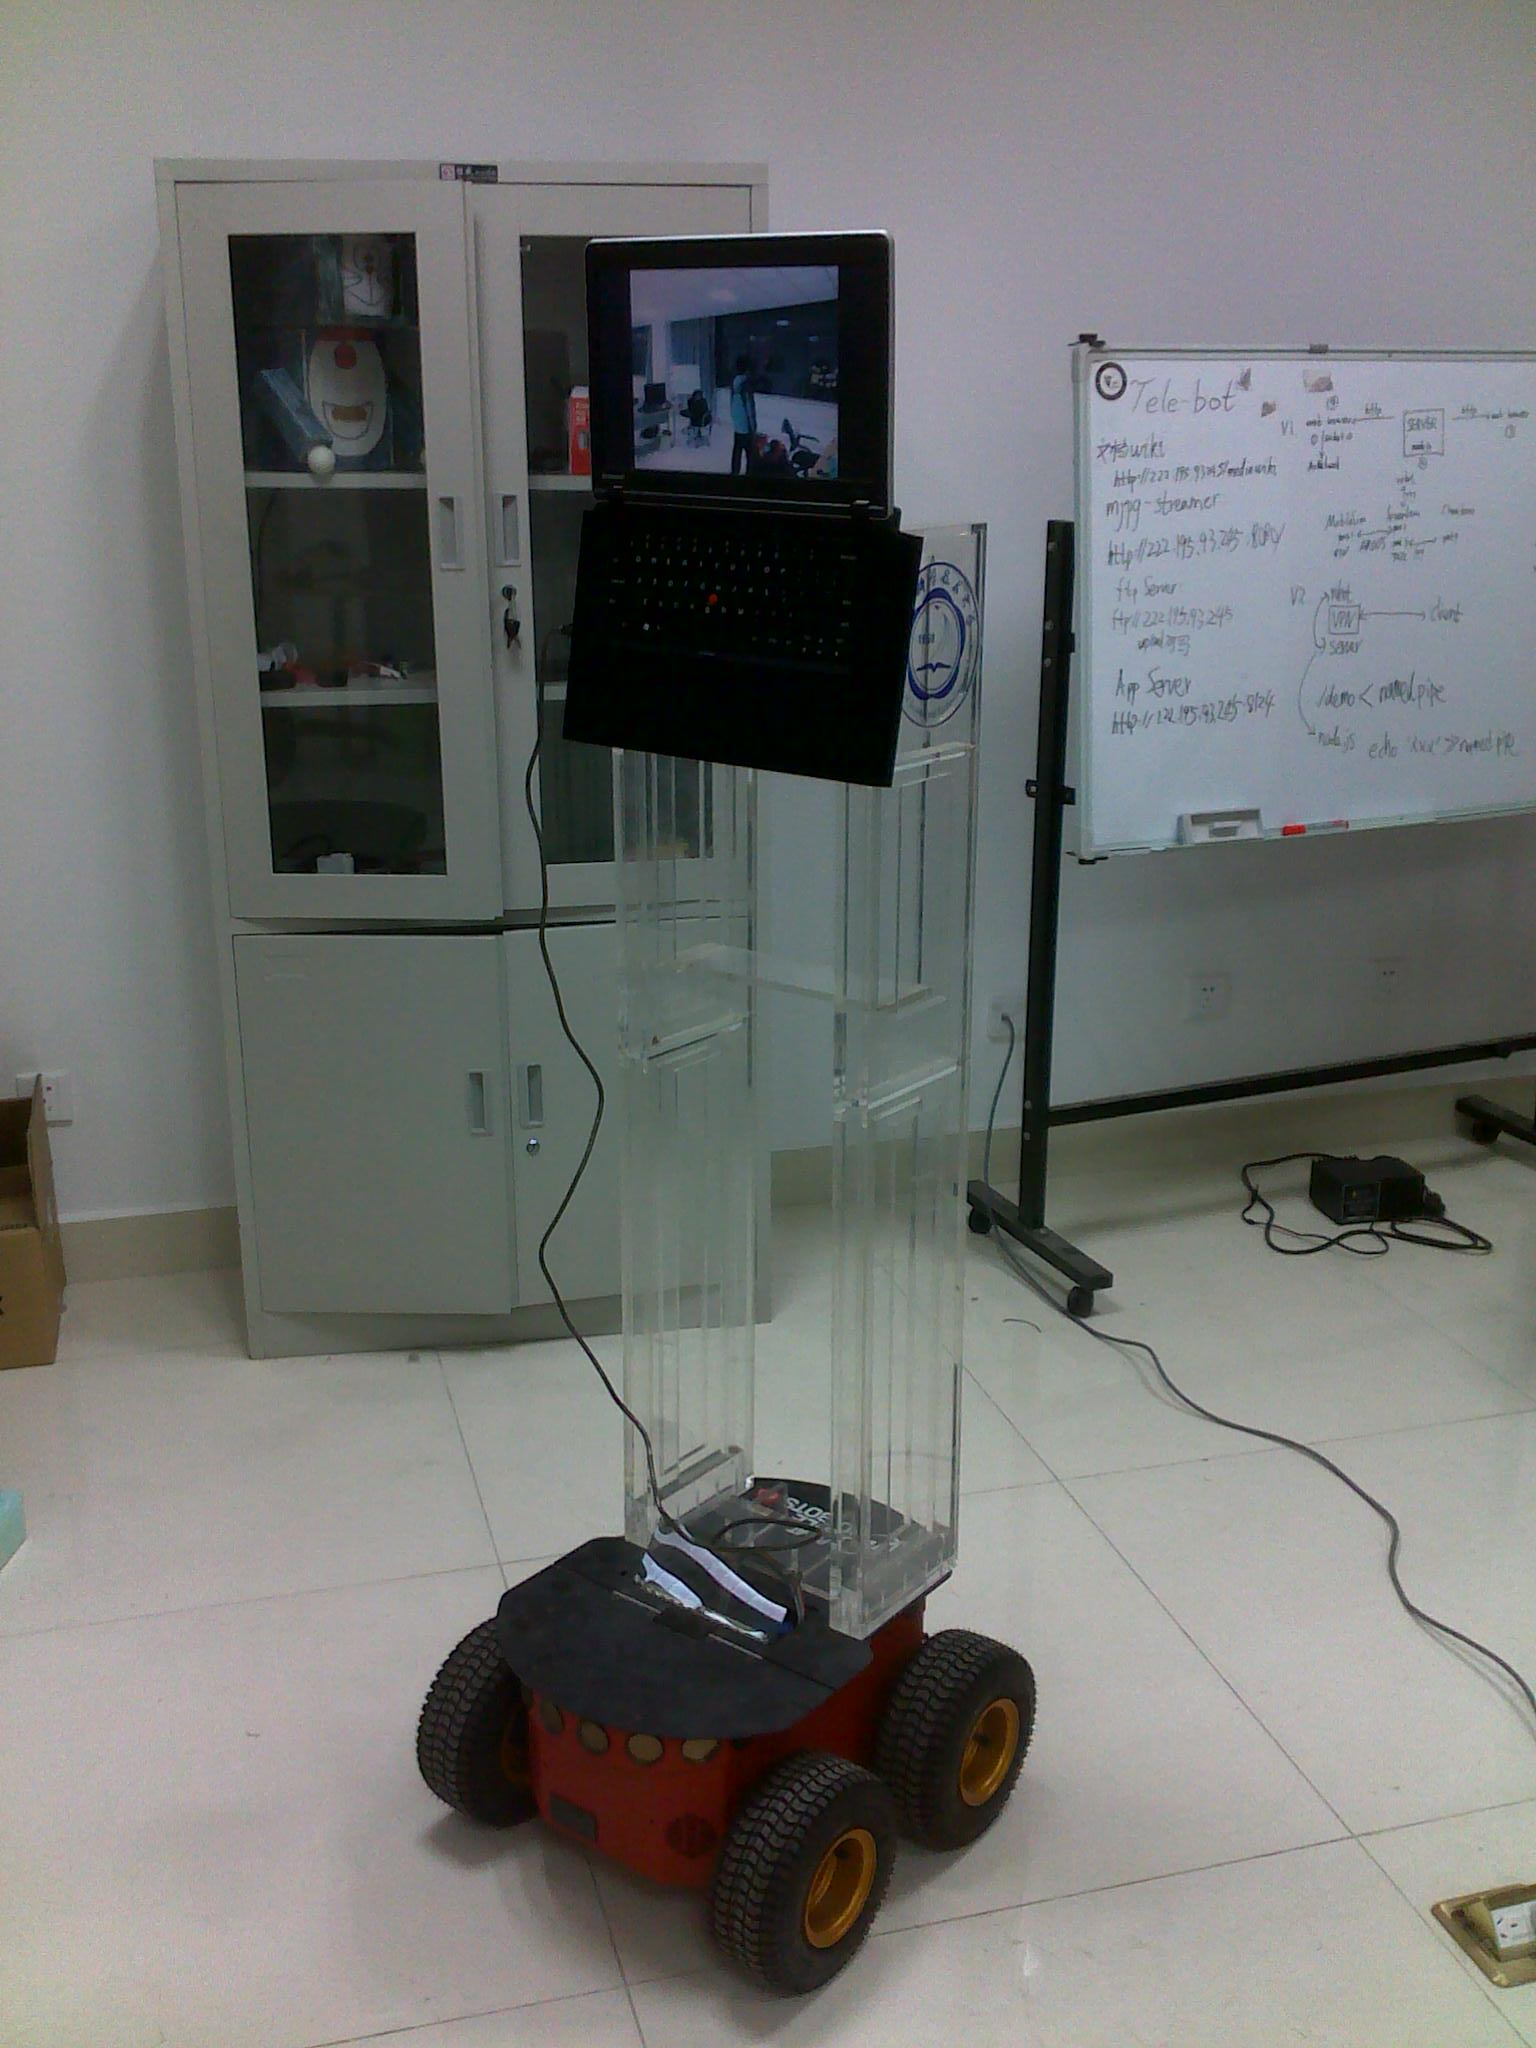
\includegraphics[width=.70\textwidth]{Figures/ch9.outlook.jpg}
        \caption{机器人外观}
        \label{fig:outlook}
\end{figure}

用户端主界面如下

\begin{figure}[h]
        \centering
                
\includegraphics[width=.70\textwidth]{Figures/ch9.ui.png}
        \caption{用户界面}
        \label{fig:UI}
\end{figure}

这是登入服务页面的效果图,用户通过点击注册来获得有权限的账号。

点击帮助按钮会提供一段视频,展示该服务的使用具体使用方法。

用户登录之后,便进入到相应的有使用权限的页面,如下图:

\begin{figure}[h]
        \centering
                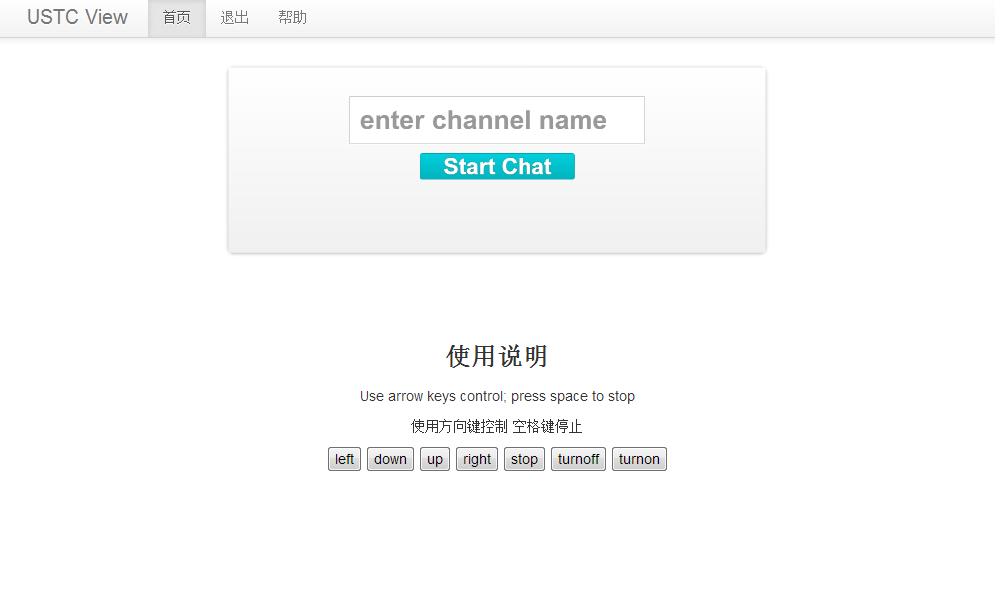
\includegraphics[width=.70\textwidth]{Figures/ch9.user.png}
        \caption{登录后界面}
        \label{fig:user}
\end{figure}

在channel name中输入机器人提供的相关channel信息,点击start即可开始音视频的通讯。
效果如下图,视频由机器人上的广角摄像头拍摄所得。

\begin{figure}[h]
        \centering
                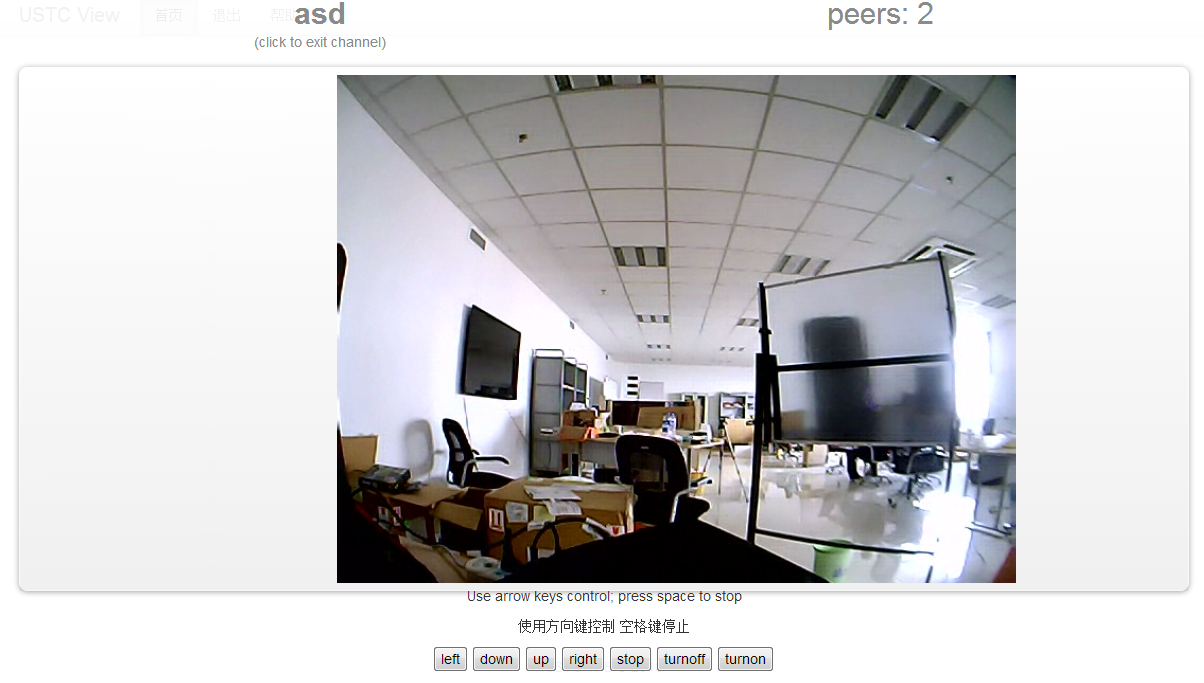
\includegraphics[width=.70\textwidth]{Figures/ch9.view.png}
        \caption{远程呈现}
        \label{fig:view}
\end{figure}

在该页面上,敲击方向键上下左右来控制移动,或者通过直接点击面板上的按钮来实现。


%%%%%%%%%%%%%%%%%%%%%%%%%%%%%%%%
% Appendices are set up same as chapters
\chapter{参考资料}
\label{cha:resources}

http://zh.wikipedia.org

%Include lists of human, institutional and vendor resources here with contact information. This is not for direct citations, which go on the Bibliography.


%%%%%BEGIN BIBLIOGRAPHY%%%%%%%%%
% This is a two-step process in which you first create a ".bib" file, which is processed
% by bibtex into a ".bbl" file for loading into the document. 
% Many online journals and databases now have a feature to automatically download Bib
% citations.  BibDesk is a handy (free) program for Macintosh for managing them.
% EndNote and Refworks (is free to Stanford students) are good alternatives.
\bibliographystyle{plainurl310}     %Modified slightly from plainurl.bst 
\bibliography{me310reportfall}  % Look for file called "me310report.bib" 
%
% Alternatively, you can create your own bibliography list by hand.
% In that case, comment out the last line above and replace with  \input{OurBibFile} 
%%%%%END BIBLIOGRAPHY%%%%%%%%%

%%%%%BEGIN APPENDIX SECTIONS%%%%%%%%%%%%%%%
\appendix
\chapterstyle{default}
 % Appendices are set up same as chapters
% \chapter{Moderator Prototype Data}
% \label{sec:Appendix1}
% Adapted from Autodesk Fall 2007-08 \cite{Autodesk2008Fall}.

% \begin{figure}
%       \centering
%               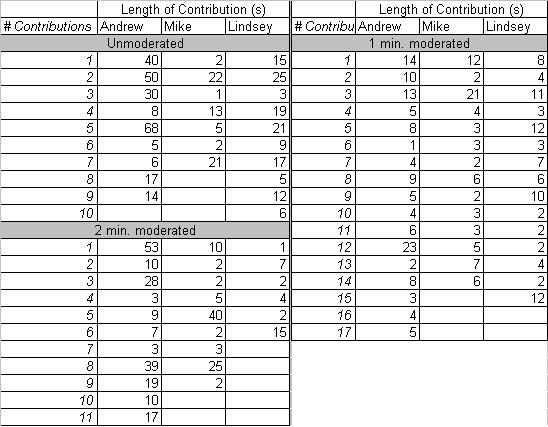
\includegraphics[width=0.75\textwidth]{Figures/Appendix1/moderatordata.JPG}
%               %Note the use of a short caption tag for the list of figures.
%       \caption[test meetings data]{Length and number of contributions collected from recorded moderator test meetings}
%       \label{fig:moderatordata}
% \end{figure}
\chapter{CC BY-SA 3.0 License}
\subsection*{Attribution-ShareAlike 3.0 Unported  (CC BY-SA 3.0) }
Disclaimer

  The Commons Deed is not a license. It is simply a handy reference for understanding the Legal Code (the full license) — it is a human-readable expression of some of its key terms. Think of it as the user-friendly interface to the Legal Code beneath. This Deed itself has no legal value, and its contents do not appear in the actual license. 


  Creative Commons is not a law firm and does not provide legal services. Distributing of, displaying of, or linking to this Commons Deed does not create an attorney-client relationship. 
 This is a human-readable summary of the Legal Code (the full license).  Disclaimer  This license is acceptable for Free Cultural Works. \subsubsection*{You are free:}
\begin{itemize}
\item \textbf{to Share}
--- to copy, distribute and transmit the work 
\item \textbf{to Remix}
--- to adapt the work 
\item  to make commercial use of the work 

\end{itemize}
\subsubsection*{Under the following conditions:}
\begin{itemize}
\item 

 \textbf{Attribution}
 ---  You must attribute the work in the manner specified by the author or licensor (but not in any way that suggests that they endorse you or your use of the work).   


%  \textbf{ Attribute this work: }
% \\ 
%     Information 
%  What does ``Attribute this work'' mean?  The page you came from contained embedded licensing metadata, including how the creator wishes to be attributed for re-use. You can use the HTML here to cite the work. Doing so will also include metadata on your page so that others can find the original work as well. 
\item 

 \textbf{Share Alike}
 --- If you alter, transform, or build upon this work, you may distribute the resulting work only under the same or similar license to this one.  


\end{itemize}
\subsubsection*{ With the understanding that: }
\begin{itemize}
\item \textbf{Waiver}
 --- Any of the above conditions can be waived if you get permission from the copyright holder. 
\item \textbf{Public Domain}
 --- Where the work or any of its elements is in the public domain under applicable law, that status is in no way affected by the license. 
\item \textbf{Other Rights}
 --- In no way are any of the following rights affected by the license: \begin{itemize}
\item  Your fair dealing or fair use rights, or other applicable copyright exceptions and limitations; 
\item  The author's moral rights; 
\item  Rights other persons may have either in the work itself or in how the work is used, such as publicity or privacy rights. 

\end{itemize}
\end{itemize}
       % There could be multiple appendix files like this
 %%%%%END APPENDIX SECTIONS%%%%%%%%%%%%%%%
 
\end{document}

